\newpage
\appendix
\section{The alternative CT18Z global fit
\label{sec:AppendixCT18Z}
}
%
% % % % A.1
%

%
\begin{figure}[b]
	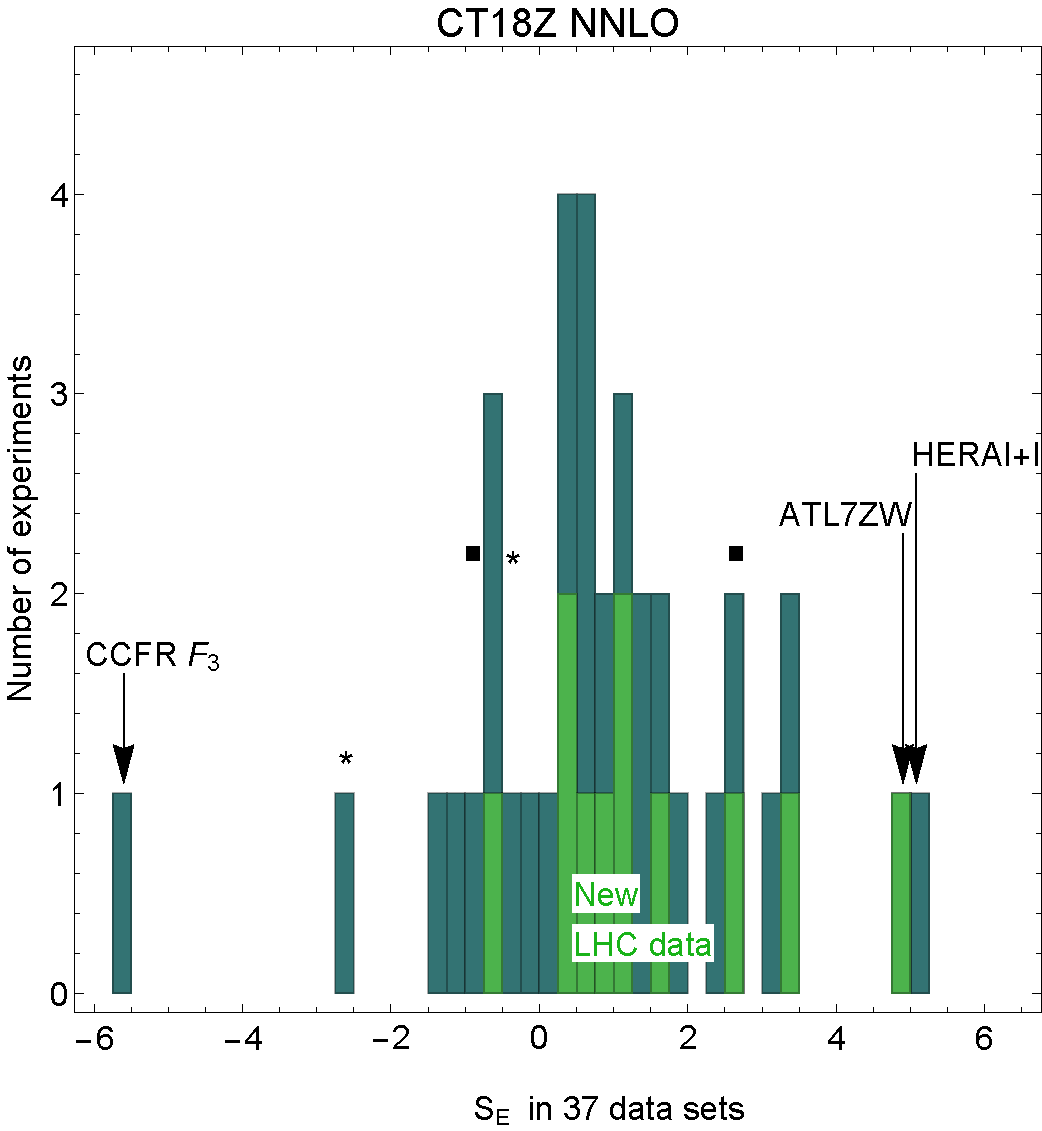
\includegraphics[width=0.49\textwidth]{./fig/sqrt2chi2_ct18ZnnloCount.pdf}
	\caption{Analogous to Fig.~\ref{fig:sn_ct18}, the effective Gaussian variable ($S_E$) distribution of all CT18Z data sets. Two squares and two stars indicate the $S_E$ values
	for the NuTeV dimuon and CCFR dimuon experiments, respectively.
\label{fig:sn_ct18z}}
\end{figure}

In this appendix, we describe a series of fits leading to the CT18Z PDFs that provide a distinct alternative to the primary result of this analysis, CT18 NNLO. 
While CT18Z NNLO achieves a comparable level of success in describing the CTEQ-TEA data, producing $\chi^2/N_\mathit{pt}\! =\! 1.19$ as opposed to $\chi^2/N_\mathit{pt}\! =\! 1.17$
for the default CT18 NNLO fit, the quality of the agreement for specific data sets undergoes a number of changes. The can be seen in part by comparing the distribution of $S_E$ values
obtained for CT18Z in Fig.~\ref{fig:sn_ct18z} with what we presented for CT18 in Fig.~\ref{fig:sn_ct18}.
%
The inclusion of the ATLAS 7 TeV $W/Z$ data (or, ATL7ZW data, with
CTEQ experimental ID=248) in CT18Z causes an upward shift of $S_E$ (or $\chi^2_E/N_{pt,E}$) for a number of experiments, notably for the dimuon data
from NuTeV (Exp.~IDs=124, 125) and CCFR (Exp.~IDs=126, 127), indicating that the ATL7ZW data is in some disagreement with these other data sets.

In Sec.~\ref{sec:alt}, we pointed out that we release two intermediate fits, CT18A (with addition of ATL7ZW data only) and CT18X (with a specially-chosen factorization scale in DIS cross sections).  
Compared to CT18A and X, the CT18Z PDFs produce maximal changes away from CT18 in the PDFs and their moments, the parton luminosities, and standard-candle predictions: those can be viewed in Figs.~\ref{fig:PDFbands1}, \ref{fig:DBandSBbands}, \ref{fig:DBandSBbands2}, \ref{fig:lumia}, \ref{fig:corr_ellipse1}, and \ref{fig:corr_ellipse2}.


We will now look into the accretion of the modifications that led from CT18 to CT18Z NNLO in more detail. The role of the ATL7ZW and CDHSW experiments is reviewed in Sec.~\ref{sec:CT18Z_changes}. Sec.~\ref{sec:CT18ZvsCT18} summarizes the key differences between CT18, A, X, and Z PDFs, while the plots of error bands for CT18A and X NNLO and NLO PDFs are included in supplemental material. 
The agreement with the ATL7ZW data is explored in Sec.~\ref{sec:CT18Z_qual}. 
In Sec.~\ref{sec:LMCT18Z}, we examine $\chi^2$ scans to extract detailed information on the redistribution of constraints on the PDFs inside the CT18Z global fit, as well as on the CT18Z predictions for $\alpha_s(M_Z)$ and $m_c$.

The physics conclusions presented here have been verified using
several independent techniques. Initially, projections of the likely
impact of the data sets on the PDFs were obtained by applying the fast
Hessian techniques, \texttt{PDFSense}/$L_2$
sensitivity \cite{Wang:2018heo,Hobbs:2019gob}
and \texttt{ePump} \cite{Hou:2019gfw}, by starting from theoretical
predictions based on the previous \CTHERAII~ NNLO
PDFs \cite{Hou:2016nqm}. At this stage, we discovered that
the \texttt{ePump} and \texttt{xFitter} programs produce very
different results when profiling the ATL7ZW data. This discrepancy
is addressed in App.~\ref{sec:Appendix4xFitter}.
As a part of the fitting itself, we repeated
some fits multiple times while either constraining the PDFs at
specific values using Lagrange Multipliers (LM) or varying the
statistical weights of ATL7ZW and other data sets to explore their
mutual consistency within the approach by Collins and
Pumplin \cite{Collins:2001es}. All these methods render a coherent
physics picture that will be now summarized. 

% ~ ~ ~ ~ ~ ~ ~ ~ ~ ~ ~ ~ ~ ~ ~ ~ ~ ~ ~ ~ ~ ~ ~ ~ ~ ~ ~ ~ ~
%
\subsection{Alterations to data sets and theoretical settings}
\label{sec:CT18Z_changes}

\subsubsection{Modified data selection}
%
Let us first address some questions arising in the description
of two data sets: ({\it i}) the recent 7 TeV Drell-Yan data taken by ATLAS for the rapidity distributions the inclusive production
of the $W$ and $Z$ bosons (ATL7ZW, Exp.~ID=248); and ({\it ii}) the $F^p_2$, $xF^p_3$ DIS structure function information
extracted by CDHSW from $\nu$-Fe data (Exp.~IDs=108, 109).

\begin{figure}[tb]
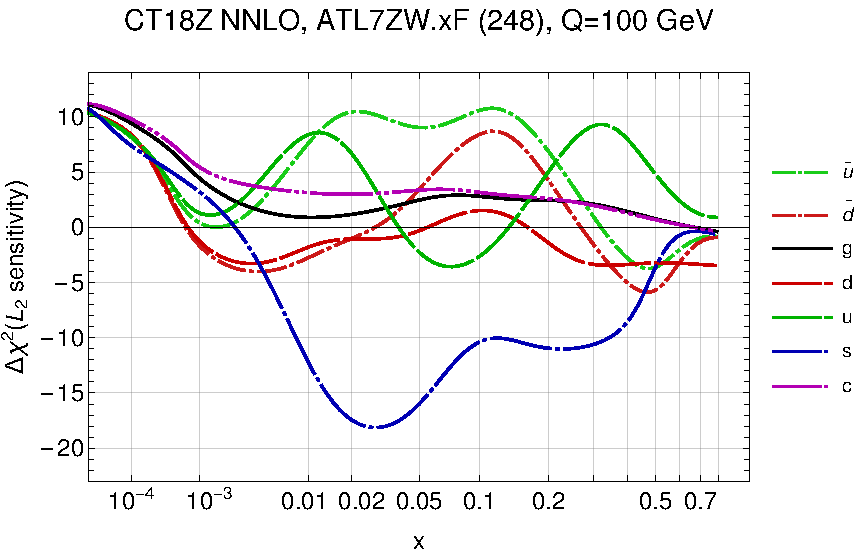
\includegraphics[width=0.7\textwidth]{./fig/AXZ/248_ct18znn_L2_q100_Sf_1.pdf}
%\hspace*{-2cm}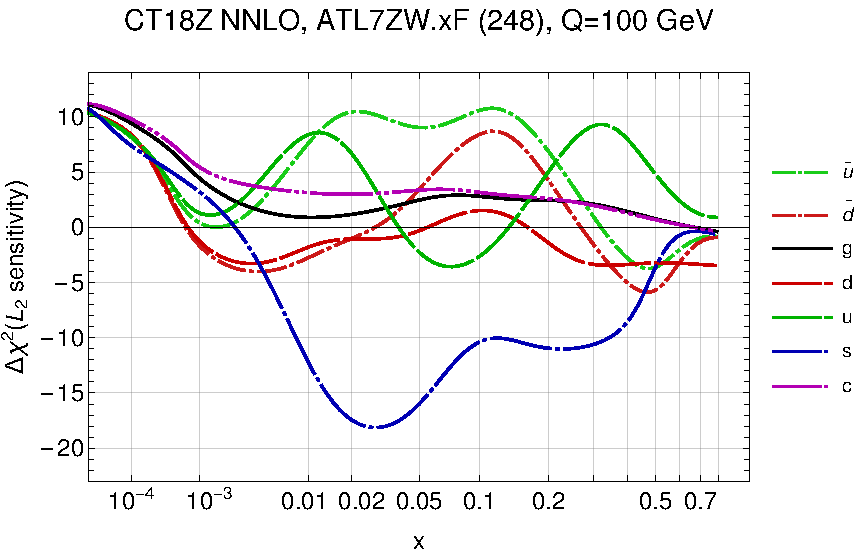
\includegraphics[width=0.7\textwidth]{./fig/AXZ/248_ct18znn_L2_q100_Sf_1.pdf}
%\hspace*{1.2cm}\includegraphics[width=0.9\textwidth]{./fig/AXZ/248_ct18znn_q100_Sf_2.pdf}
\vspace{-2ex}
\caption{
	The $L_2$ sensitivity of the ATL7ZW data to the PDFs of
	several individual parton flavors. The pull on the strangeness distribution,
	$s(x,Q)$, is particularly large, peaking at $S_{s,\mathit{L2}}\! \sim\! -20$
	for $x\!\sim\! 0.02-0.05$; although opposing pulls on the $d$-, $\bar{u}$-,
	and $\bar{d}$-quark PDFs are also significant in a similar region of $x$.
}
\label{fig:L2_248}
\end{figure}


\begin{figure}[htbp]
        \begin{center}
                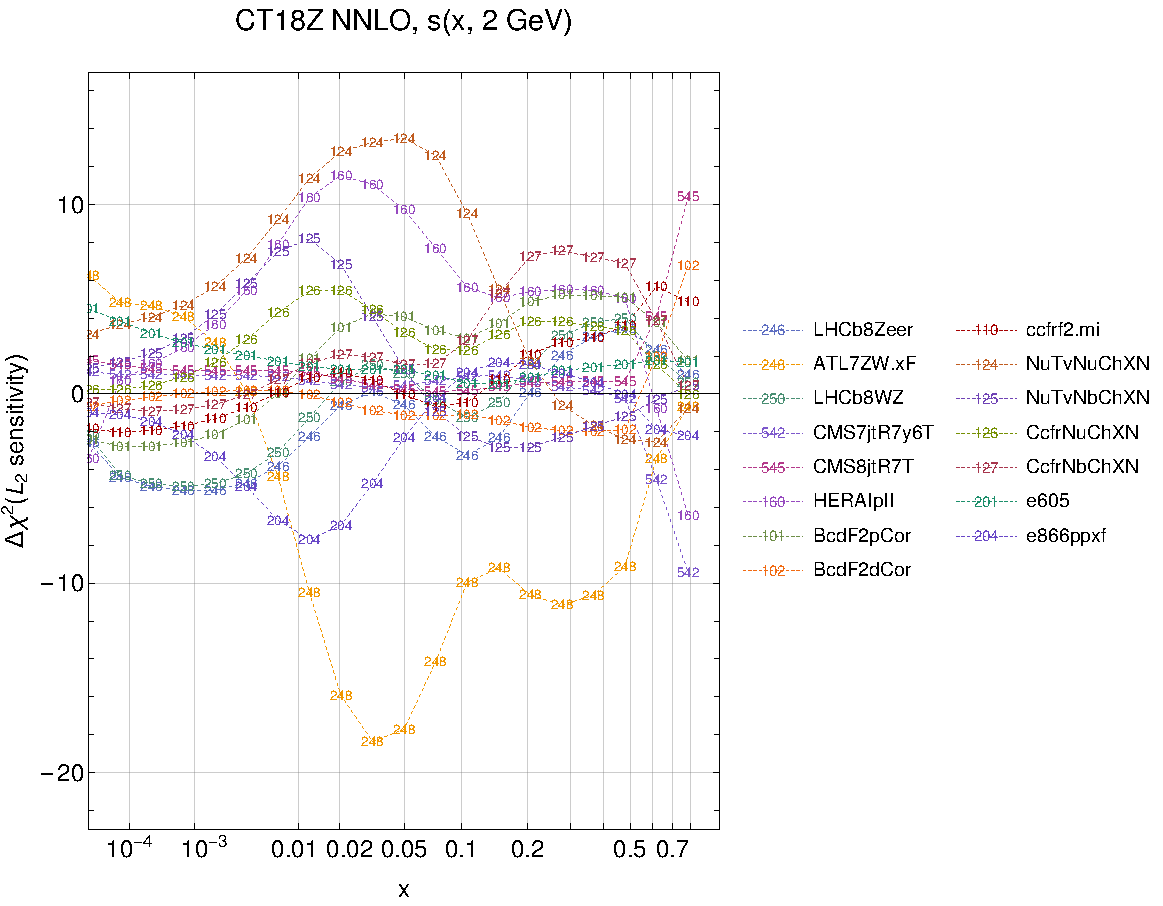
\includegraphics[width=0.95\textwidth]{./fig/Sens/ifl3_ct18znn_L2_q2_Sf_1.pdf}
        \end{center}
        \vspace{-2ex}
        \caption{
		The $L_2$ sensitivity of the data fitted in CT18Z to the $x$-dependent
		strange PDF at $Q\!=2$ GeV. Given that the fitted behavior for
		$R_s(x,Q)$ is substantially driven by $s(x,Q)$, the information
		shown here is complementary to the LM scans in Fig.~\ref{fig:lm_rsz}.
        }
\label{fig:L2sZ}
\end{figure}

{\bf ATLAS 7 TeV Inclusive $W/Z$-production data.}
%
%
Regarding case ({\it i}), the ATL7ZW data set is seen as providing
important information on the structure of the light-quark nucleon sea,
and, in particular, favoring an enhanced value for the strangeness
suppression factor, $R_s(x,Q)$ of Eq.~(\ref{eq:Rs})
compared to what has been found in the past global analyses
dominated by the DIS data.
The sensitivity analysis indicates that, while
the correlation cosines of the ATL7ZW measurements
with respect to various PDF flavors are quite modest
(typically, $|\cos \phi|\! <\! 0.6$), the sheer precision of the
ATL7ZW data creates a pronounced
pull on all light-antiquark flavors: $\bar u$, and $\bar d$, and
especially $\bar s$. For example, the pulls are revealed by the charts
showing $L_2$ sensitivities of ATL7ZW data to various CT18Z PDF flavors
in Fig.~\ref{fig:L2_248}. The strong positive pull on $s(x,Q)$
revealed by the corresponding negative $S_{L2,E}$ for $s(x,Q)$
at $x=0.01-0.1$ in Fig.~\ref{fig:L2_248} must be compensated in the
global fits by the
opposing pulls from other experiments. For example, we can compare
the Hessian estimates of the pulls on $s(x,Q=2\mbox{ GeV})$
by plotting the respective sensitivities for individual
experiments in Fig.~\ref{fig:L2sZ}. It is obvious that the prominent
negative pull on $\Delta \chi^2$ from ID=248 at $x=0.03$ is opposed by
the positive pulls from NuTeV (Exp.~ID=124, 125) and CCFR
(Exp.~ID=126, 127) dimuon SIDIS, and, also very prominently, the
inclusive HERAI+II data (Expt.~ID=160). On the other hand, the
fixed-target E866 Drell-Yan data on the $pp$ target (Expt.~ID=204)
weakly pulls in the same direction as ATL7ZW, although at smaller
$x \approx 0.01$.

While the $L_2$ sensitivity estimates contributions
to $\chi^2$, tensions with the ATL7ZW data are also revealed by other
statistical indicators, such as an effective Gaussian variable $S_E$
for experiment $E$ that quantifies how the change in $\chi^2_E$
compares to the respective statistical uncertainty. By this measure, 
the Hessian updating study \cite{Hou:2019gfw} based on \texttt{ePump} 
found that including the ATL7ZW data with
increasing statistical weights into the CT18 fit strongly increases
$S_E$ values for the NuTeV $\nu$ SIDIS (Exp.~ID=125),
the E866 $\sigma_{pd}/(2\sigma_{pp})$ Drell-Yan data (Exp.~ID=203),
and the CMS 7 TeV electron asymmetry data (Exp.~ID=267),
cf.~Fig.~25 of~\cite{Hou:2019gfw}. This change is accompanied by
modifications in the $s$-quark PDF and $\bar{d}/\bar{u}$ PDF ratio,
cf.~Fig.~26 of the same reference. Finally, we observe mild
suppression of $g(x,Q)$ at $x \gtrsim 10^{-2}$ after including the
ATL7ZW data set.

{\bf CDHSW data.}
Our LM scans, like the ones presented in Fig.~\ref{fig:LMg18} and the
$L_2$ sensitivity plot in Fig.~\ref{fig:L2glu}, reveal
that the CDHSW measurements of deep inelastic scattering
in charged-current neutrino interactions on iron
(Exp.~IDs=108 \cite{Berge:1989hr}, 109 \cite{Berge:1989hr})
are sensitive to the gluon distribution at $x > 0.2-0.5$ via $Q^2$
distributions of their cross sections. At $x <0.4$, the logarithmic
slopes of the structure functions $F_2$ and $xF_3$ measured by CDHSW
and CCFR are different, cf. Figs.~8.3 and 8.4 in
Ref.~\cite{Seligman:1997fe}, with CDHSW structure functions preferring
a harder $g(x,Q\!=\!100\,\mathrm{GeV})$ at $x\!\approx\!0.2$, but a softer
gluon at $x\!\gtrsim\!0.5$ --- similarly to the CDF Run-2 jet data
(Exp.~ID=504). It has been known that unresolved experimental issues may exist
in the CDHSW analysis~\cite{Barone:1999yv}, and nuclear corrections
may be non-negligible for the iron target. Thus,
one may wonder how the PDFs would change if
these two CDHSW data sets are excluded. This question was addressed
using  \texttt{ePump} in Ref.~\cite{Hou:2019gfw}, as well as by performing a special fit named
``CT18mCDHSW'' ({\it i.e.}, CT18 ``minus'' CDHSW), in which
the two CDHSW data sets were removed from the CT18 global data.

The plots of PDF error bands from the CT18mCDHSW NNLO fit, included in
the supplemental material, show that removing CDHSW data leads to a
slight reduction in the gluon PDF at $x=0.1-0.5$, combined with a
slight increase in the gluon PDF uncertainty, and compensating
increases in the $u$ and $d$ PDFs in the same $x$ region. 

\subsubsection{The $x_B$-dependent scale and modified global fits}
%
Another point of potential concern is the residual dependence on QCD
cross sections on the renormalization and factorization scales, which
we find to be non-negligible in some experiments, compared to the
latest experimental uncertainties, even when NNLO theoretical
expressions for QCD cross sections are used. In particular, by
evaluating the NNLO DIS cross sections at a carefully chosen
factorization scale $\mu_{F,x}$
dependent on Bjorken $x_B$ in Table~\ref{tab:AXZ},
we moderately improve agreement with HERA DIS cross sections:
the respective $\chi^2$ improves by 40 units
($\chi^2(\mbox{CT18})=1408$, $\chi^2(\mbox{CT18Z})=1378$ for
$N_{pt}=1120$ data points), and it can be improved by another 30 units
by increasing the statistical weight of the inclusive HERA data to 10 as in
the right Fig.~\ref{fig:saturation}. With this scale choice, we also obtain
larger PDFs for the gluon and strangeness PDFs at momentum fractions $x$
below 0.05, cf. left Fig.~\ref{fig:saturation}. At the same time,
$g(x,Q)$ and $s(x,Q)$ are reduced from $x=0.2$ to 0.4-0.5 to preserve
the sum rules.

Therefore, three modifications in the global fitting framework -- using
the $\mu_{F,x}$ scale in DIS, excluding the CDHSW data sets, and
adding the ATLAS7ZW data -- add up to suppress the gluon PDF at
$0.005 \lesssim x \lesssim 0.3$, across most of the interval
of $x$ relevant for the LHC
Higgs production via $gg$ fusion. Their combination also produces a
substantial increase of $s(x,Q)$ at all $x$. 

As discussed in Sec.~\ref{sec:alt}, this combination is adopted to
produce the CT18Z NNLO PDFs. The intermediate PDFs, CT18A and CT18X,
implement only the ATL7ZW data in the $66 < Q < 116$ GeV region (34
data points) or only the DIS scale $\mu_{F,x}$, as
indicated in Table~\ref{tab:AXZ}. [The low-luminosity
($35\, {\rm pb}^{-1}$) sample of the ATLAS 7 TeV  $W^\pm$ and $Z$
cross section data  (Exp.~ID=268) is removed from the CT18A and Z fits
to avoid double counting.]

\subsection{Comparisons between the four PDF ensembles}
\label{sec:CT18ZvsCT18}
%

The supplemental material includes a series of figures comparing the NNLO and NLO PDF uncertainty bands for CT18, A, X, and Z PDF flavors. The main characteristics of these comparisons can be distilled as follows.

\begin{enumerate}
\item {\bf $g(x,Q)$:} By comparing the PDF uncertainty bands for CT18,
CT18A, and CT18Z, on one hand, and CT18, CT18X, and CT18Z, on the
other hand, it is clear the bulk of the variation of CT18Z away from
CT18 is due to the modified DIS scale choice, $\mu_{F,x}$, with only
weaker changes resulting from the interplay of the removal of CDHSW
and inclusion of the ATL7ZW measurements. The deviations from CT18
are generally smaller at NLO, with the exception of the very low-$x$
region, where CT18Z and CT18X NLO ratios to CT18 are $\sim\! 50\%$ larger.
%
\item {\bf $d(x,Q)$:} In contrast to $g(x,Q)$, the sensitivity
of the Drell-Yan process to $d(x,Q)$ enhances the difference
between the CT18 and CT18A NNLO results for this flavor, realized as a
mild, $\sim\!1\%$ suppression of the central CT18A distribution for
$d(x,Q)$ relative to CT18 about $x\!\sim\!10^{-3}$, with a
few-percent reduction in the accompanying PDF uncertainty. The CT18Z
fit in this region is pulled in the opposing direction, being enhanced
by $\lesssim\!2\%$ with a comparable uncertainty for $x\!<\! 0.1$. In
the high-$x$ region,
$x \gtrsim 0.2$, the effect of fitting the ATL7ZW data
alone in CT18A NNLO boils down to a small shift in the $d(x,Q)$
uncertainty. CT18Z, in contrast, is suppressed relative to CT18 at higher values of $x$. 
The qualitative impact of fitting $d(x,Q)$ at NLO, as opposed
to NNLO, is fairly weak, being felt mostly at lower $x\!\lesssim\!
10^{-3}$.
%
\item {\bf $u(x,Q)$ and $\bar u(x,Q)$:} Here, the remarkable property
is the extent to which the deviations of CT18Z NNLO away from CT18
NNLO are driven by the modifications in CT18X, as attested by the very
close agreement between the central PDFs and uncertainties 
for CT18Z and X. The weak suppression of $\bar{u}(x,Q)$
in CT18A NNLO is almost entirely nulled once the DIS-scale
choice found in CT18X is implemented in CT18Z on top of the ATL7ZW measurements.
%
\item {\bf $s(x,Q)$ and $R_s(x,Q)$:} We have noted already
that the introduction of the ATL7ZW data in
CT18A/Z NNLO fits leads to a demonstrable enhancement of $s(x,Q)$ over
CT18, while the scale choice in CT18X mildly suppresses $s(x,Q)$ at
$0.01 \lesssim x \lesssim 0.5$ and enhances it at $x \lesssim 0.01$ and 
$x \gtrsim 0.5$. The strangeness suppression ratio, $R_s(x,Q)$,
is driven for the most part by the patterns observed for $s(x,Q)$ itself.
\end{enumerate}


\subsection{A closer look at the description of ATLAS 7 $W/Z$ data}
\label{sec:CT18Z_qual}


\subsubsection{Goodness of fit to ATL7ZW data in CT18A(Z)}
\label{sec:ATL7ZWchi2}

\begin{table}[tb]
\caption{The comparison of the $\chi^{2}$ for ATLAS 7 TeV $W/Z$ data among the QCD analysis from different groups.}
\label{tab:CMN}
\begin{tabular}{c|c|c|c|c}
\hline\hline
PDF & $N_{\mathit{pt}}$ & $\chi^{2}$ & $\chi^{2}/N_{\mathit{pt}}$ & Ref. \\
\hline
ATLAS-epWZ16 & 61 & 108 & 1.77 & \cite{Aaboud:2016btc}\\
MMHT (2019) &  61 & 106.8  & 1.76 &  \cite{Thorne:2019mpt}\\
NNPDF3.1 & 34 &  & 2.14 & \cite{Ball:2017nwa} \\
CT18A &  34  & 87.6  & 2.58 & \\
CT18Z & 34 & 88.7 & 2.61  & \\
\hline\hline
\end{tabular}
\end{table}

%
Turning now to the overall description of the ATL7ZW measurement, responsible for the strong modifications of the nucleon strangeness in CT18A/Z NNLO, we find
a significant improvement in $\chi^2$ for these data once they are actually fitted. Namely, CT18 NNLO produces a very large
$\chi^2_E/N_\mathit{pt,E}\!=\! 8.4$ ($S_E\! =\! 13.7$), which diminishes substantially to
$\chi^2_E/N_\mathit{pt,E}\!=\! 2.6$ ($S_E\! =\! 4.8$) in CT18Z NNLO, as we reported in
Table~\ref{tab:EXP_2}. We note that the corresponding values for CT18A NNLO, which deviates from
the settings of CT18 NNLO only in the implementation of the ATL7ZW data, are only a very
slight improvement over CT18Z, $\chi^2_E/N_\mathit{pt,E}\!=\! 2.6$ ($S_E\! =\! 4.7$). 
%pn 2020-02-17
We also remind the reader that the CT18A/Z fits include only 34 ATL7ZW data points in the resonance region ($66 < Q < 116$ GeV), with the rest of 61 points of the published set being less precise and contributing mostly to the reduction of $\chi^2_E/N_{pt,E}$ without really improving the PDF constraints, while also enhancing the dependence of the PDFs on NLO EW corrections in the off-resonance regions. 

In comparison, the ATLAS group themselves obtained 
$\chi^2_E/N_{\mathit{pt,E}}=108/61$ in the QCD
analysis \cite{Aaboud:2016btc} of these $W/Z$ data together with the
combined HERA I+II  \cite{Abramowicz:2015mha} by
using \texttt{xFitter}. Their fitted strangeness fraction is
$R_s=(s+\bar{s})/(\bar{u}+\bar{d})=1.13\pm0.08$ at $x=0.023$, i.e., it
is significantly larger than what we obtained in the CT18A(Z) fits. 
Similar results are confirmed by only including the ATL7ZW and HERA I+II
data in the QCD analysis of CT fitting framework. Moreover, we could get an
even better $\chi^2/N_{pt,E}$ as 1.4 and even larger $R_s$ due to the
more flexible parameterization, if the ATL7ZW data were included with an elevated statistical weight. 


\begin{figure}[t]
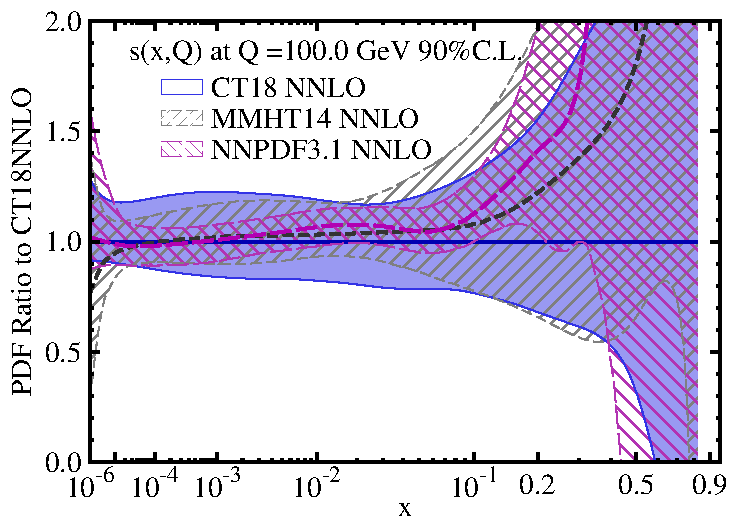
\includegraphics[width=0.7\textwidth]{fig/ATL7WZ/pdfs_CT18NNLO_MMHT2014nnlo_NNPDF31nnloas01181000_100-0GeV_A90CL_03_sqk_pdfr_cus-lin-2.pdf}
\caption{
		{\color{red}TIM: A comparison of the fitted strangeness PDF, $s(x,Q)$, at $Q\!=\!100$ GeV
		as obtained with CT18 (solid violet) as well as with MMHT14 (short-dashed gray)
		and NNPDF3.1 (long-dashed magenta). Under the latter two fits, there
		is a tendency toward enhanced strange, especially at larger values of
		$x\! >\! 0.1$.
	}}
\label{fig:s_CT-MMHT-NNPDF}
\end{figure}


%
However, we view this outcome as problematic on the grounds that
\begin{enumerate}
\item the above \texttt{xFitter} analysis strongly deemphasizes the
experiments that show tension with the ATL7ZW data, as explained in
App.~\ref{sec:Appendix4xFitter};
\item our LM scans like the ones presented in Sec.~\ref{sec:LMCT18Z}
reveal that CT fits, with their increased
flexibility compared to HERAPDF fits, become unstable or have multiple
minima when $R_s(x,Q)$ is forced to be close to 1 at $x=0.01-0.1$, as
preferred by the ATL7ZW data set; we hypothesize that the instability reflects the still weak capability of data to discriminate between the $\bar s$, $\bar d$, and $\bar u$ contributions, as has been also pointed out by ABM \cite{Alekhin:2017olj}; 
\end{enumerate}
%

Other PDF fitting groups have also investigated the ATL7ZW data. 
%pn 2020-02-17
The ABM analysis \cite{Alekhin:2017olj} has emphasized tensions between ATL7ZW, NuTeV, and NOMAD data sets, as well as strong dependence of the preferred $R_s(x,Q)$ enhancement on the flexibility of the strangeness parametrization. The 2019 MMHT analysis \cite{Thorne:2019mpt}
obtains $\chi^2_E/N_\mathit{pt,E}\!=\! 1.76$
for 61 ATL7ZW data points by (a) 
including NNLO quark-mass corrections for inclusive charged-current (SI)DIS cross sections
~\cite{Berger:2016inr,Gao:2017kkx},
which slightly improve agreement between the DIS and ATL7ZW data sets, cf. Sec.~\ref{sec:Qualitydimuon}; and (b) using flexible 6-parameter parametrizations for $d$ and $s$ quarks. 


While NNPDF did not actively fit
ATL7ZW in NNPDF3.0, which obtained $\chi_E^2/N_\mathit{pt,E}\!=\! 8.44$, they were implemented in NNPDF3.1 \cite{Ball:2017nwa},
resulting in $\chi^2_E/N_\mathit{pt,E}\!=\! 2.14$ --- very similar to the overall quality of description we
quoted above using CT18A/Z NNLO. Thus, NNPDF3.1 also observed a significant enhancement to the
fitted strange PDF at $Q\!=\!100$ GeV over a similar range of $x$.
%
{\color{red}TIM:
This enhancement is not unlike that found with MMHT14, as shown in the comparison plot of Fig.~\ref{fig:s_CT-MMHT-NNPDF},
which also reported an enlargement of the strange PDF with a somewhat broader uncertainty at high $x$.
}
%
We compare our fitted $\chi^{2}_E/N_{pt,E}$
for the ATL7ZW data to the other global fits in Tab.~\ref{tab:CMN}.


\begin{figure}[t]
	\begin{tabular}{cc}
		\subfloat[$W^-$ production]{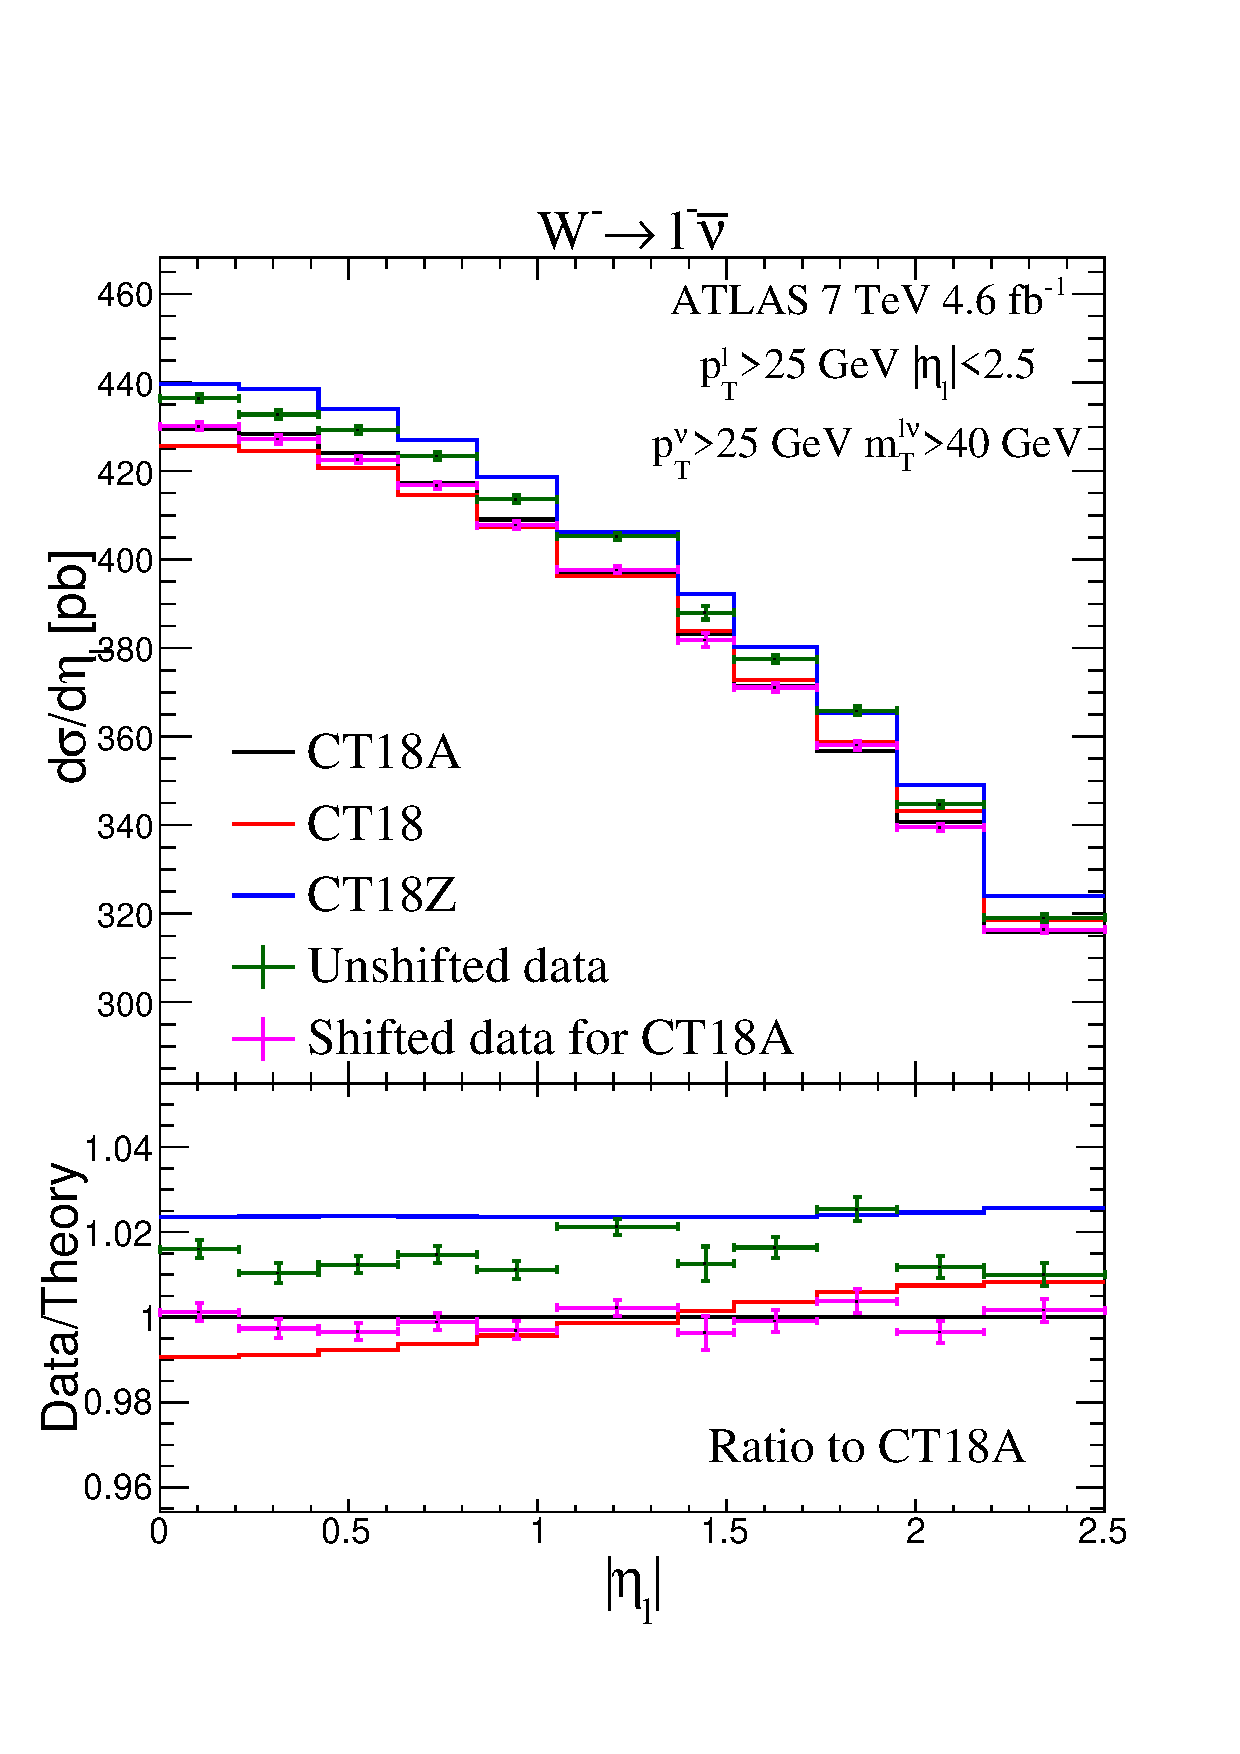
\includegraphics[width=0.35\textwidth]{fig/ATL7WZ/chisq248WmCT18A_248_CT18A.pdf}}
		\subfloat[$W^+$ production]{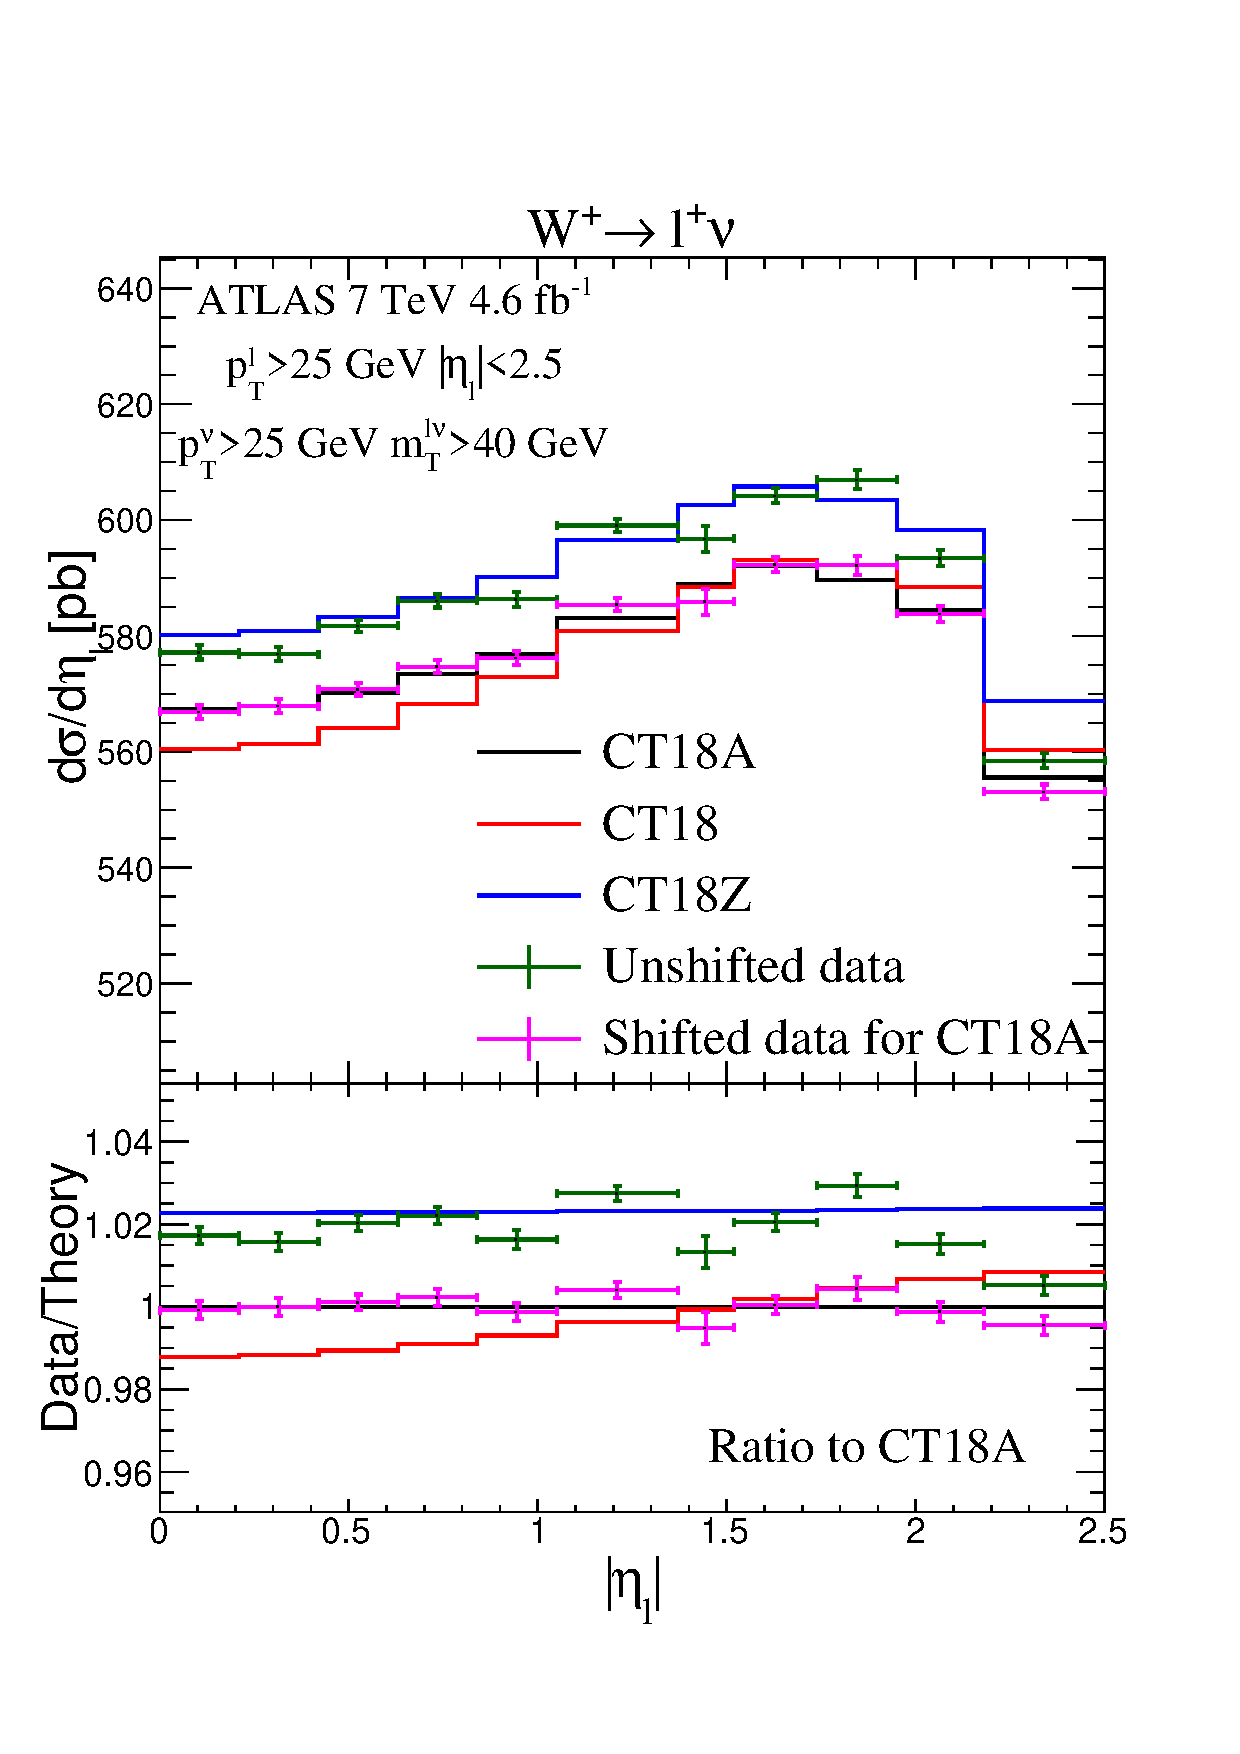
\includegraphics[width=0.35\textwidth]{fig/ATL7WZ/chisq248WpCT18A_248_CT18A.pdf}}
		\subfloat[$Z$ production]{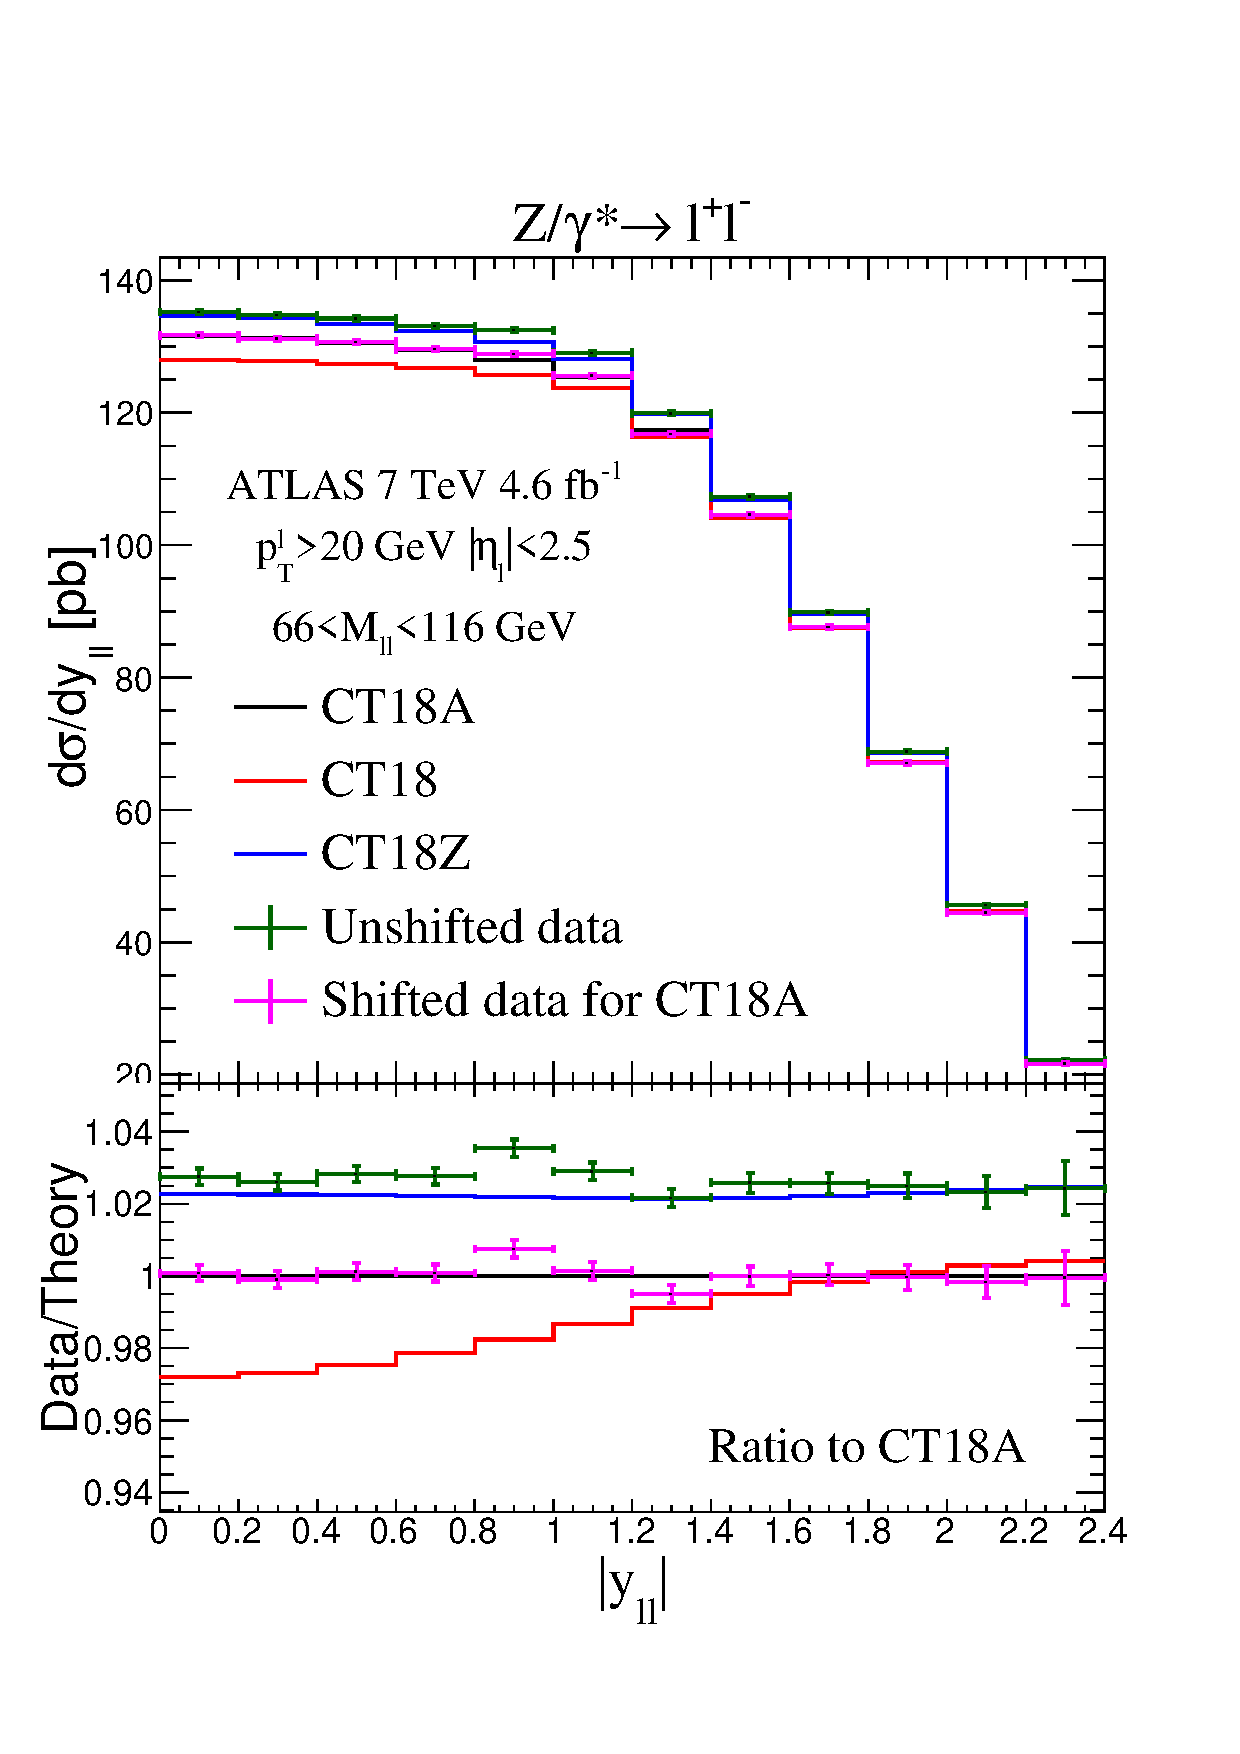
\includegraphics[width=0.35\textwidth]{fig/ATL7WZ/chisq248ZCT18A_248_CT18A.pdf}}
	\end{tabular}
	\caption{
		(a) A comparison of theoretical predictions for the ATL7ZW data based on CT18 and CT18A/Z NNLO.
		The shifted data (magenta crosses) are computed based on CT18A NNLO. The upper panels give rapidity distributions
		of the differential cross sections in $|\eta_l|$ (for the charge-current processes) or $|y_{ll}|$ (for neutral-current), while the lower
		insets show the ratios of the data and theory, normalized to CT18A theory.
	}
\label{fig:248_DT}
\end{figure}


\begin{figure}[p]
	\begin{tabular}{cc}
\subfloat[$W^-$ production]{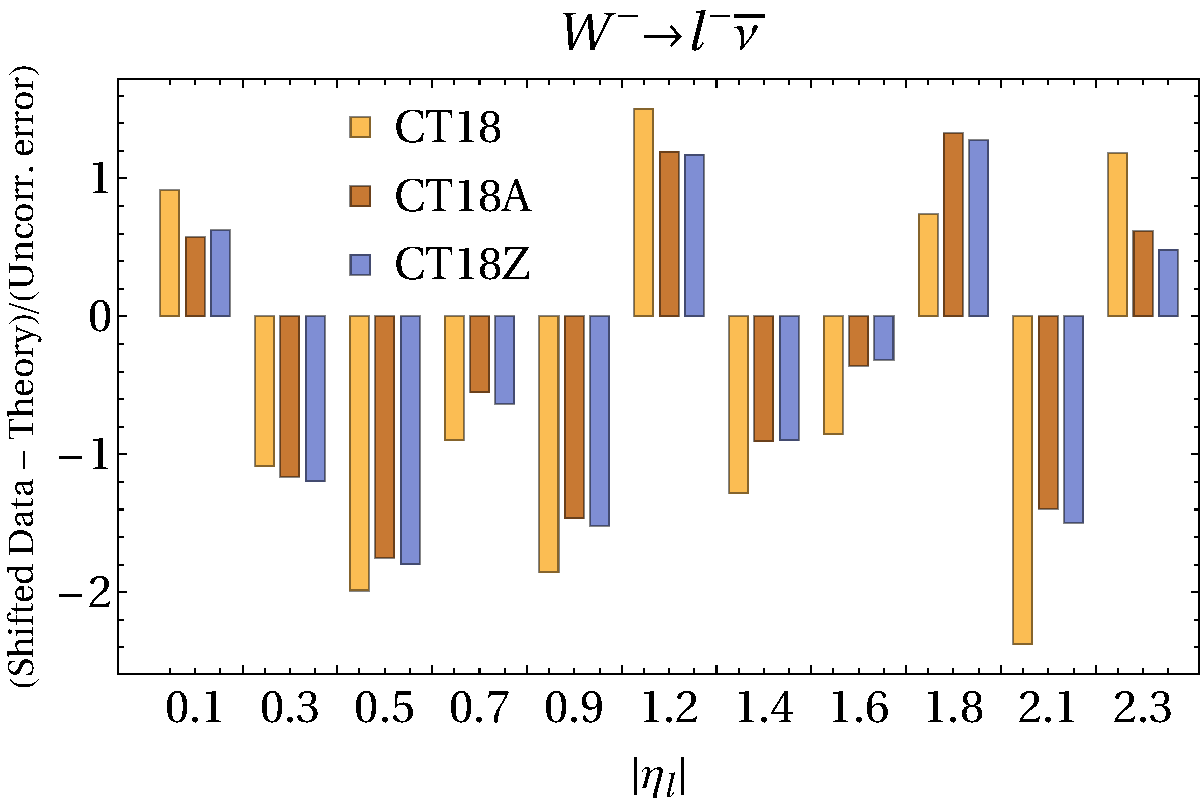
\includegraphics[width=0.49\textwidth]{fig/ATL7WZ/Residual_ATL7WZ_WmChart_shifted.pdf}}
\subfloat[$W^+$ production]{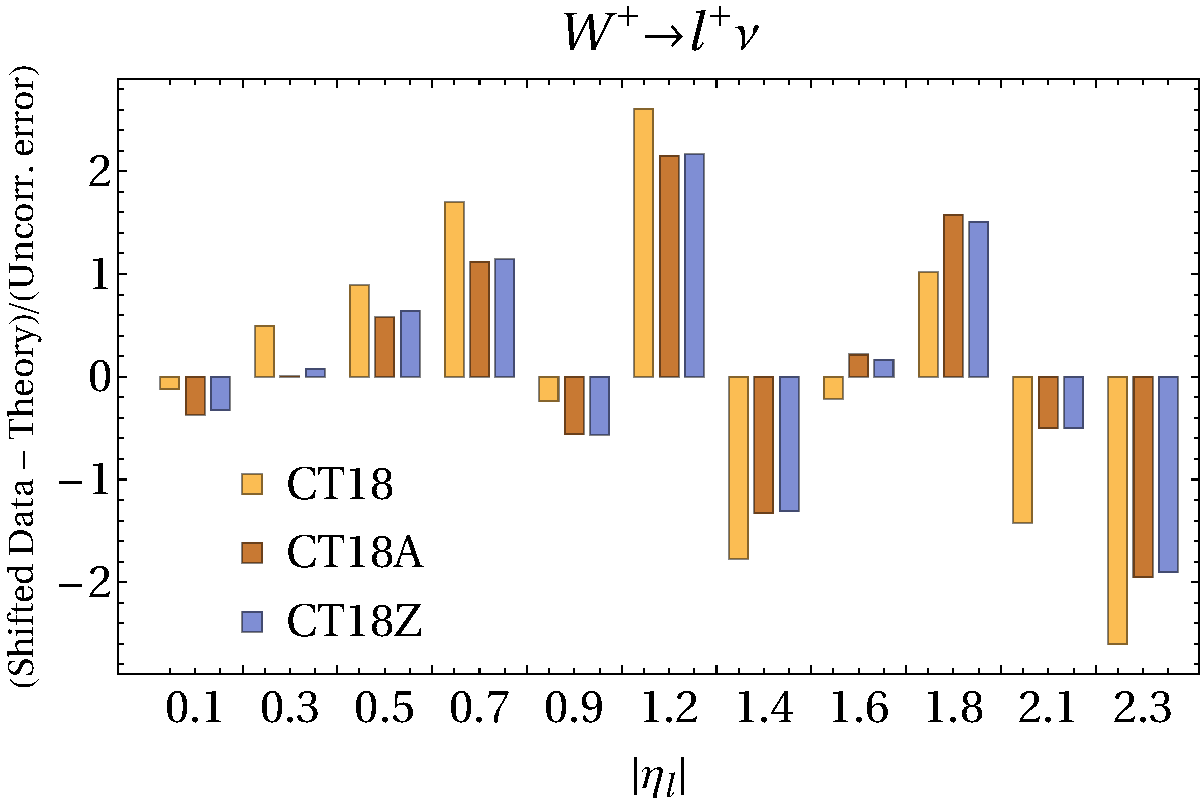
\includegraphics[width=0.49\textwidth]{fig/ATL7WZ/Residual_ATL7WZ_WpChart_shifted.pdf}}\\
\subfloat[$Z$ production]{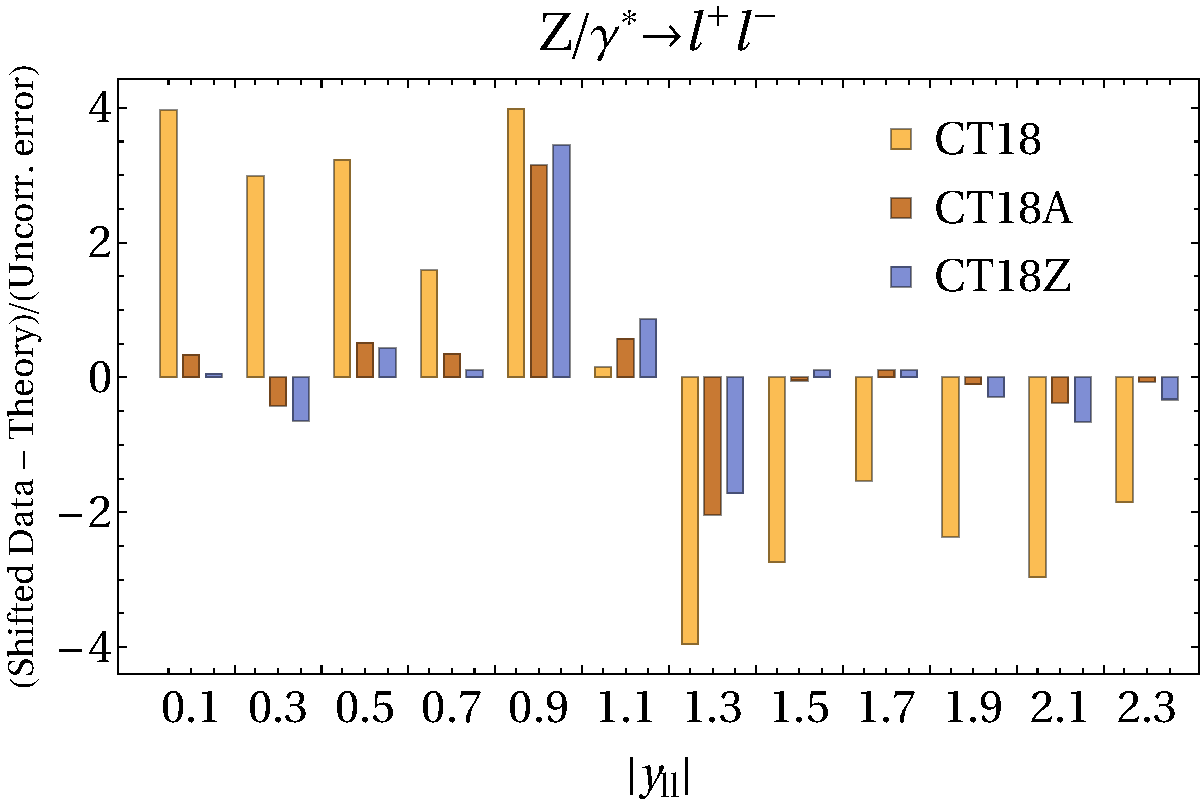
\includegraphics[width=0.49\textwidth]{fig/ATL7WZ/Residual_ATL7WZ_ZChart_shifted.pdf}}
	\end{tabular}
	\caption{
		Bin-by-bin shifted $\mathrm{Theory}\!-\!\mathrm{Data}$ residuals computed based on CT18(A/Z) for each of the three ATL7ZW processes shown in Fig.~\ref{fig:248_DT}. 
	}
\label{fig:248_res}
\end{figure}

\begin{figure}[p]
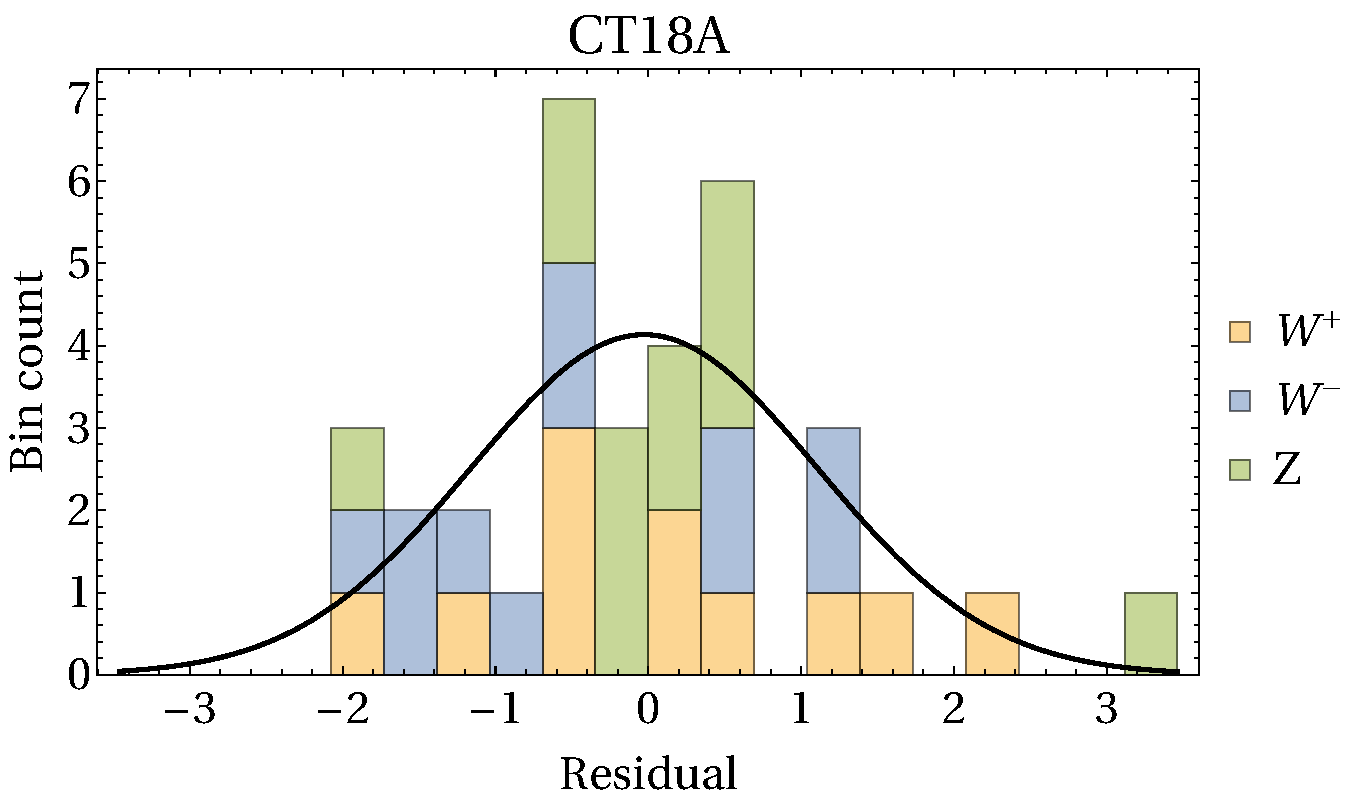
\includegraphics[width=0.49\textwidth]{fig/ATL7WZ/pResidual_CT18A_ATL7WZ.pdf}\quad 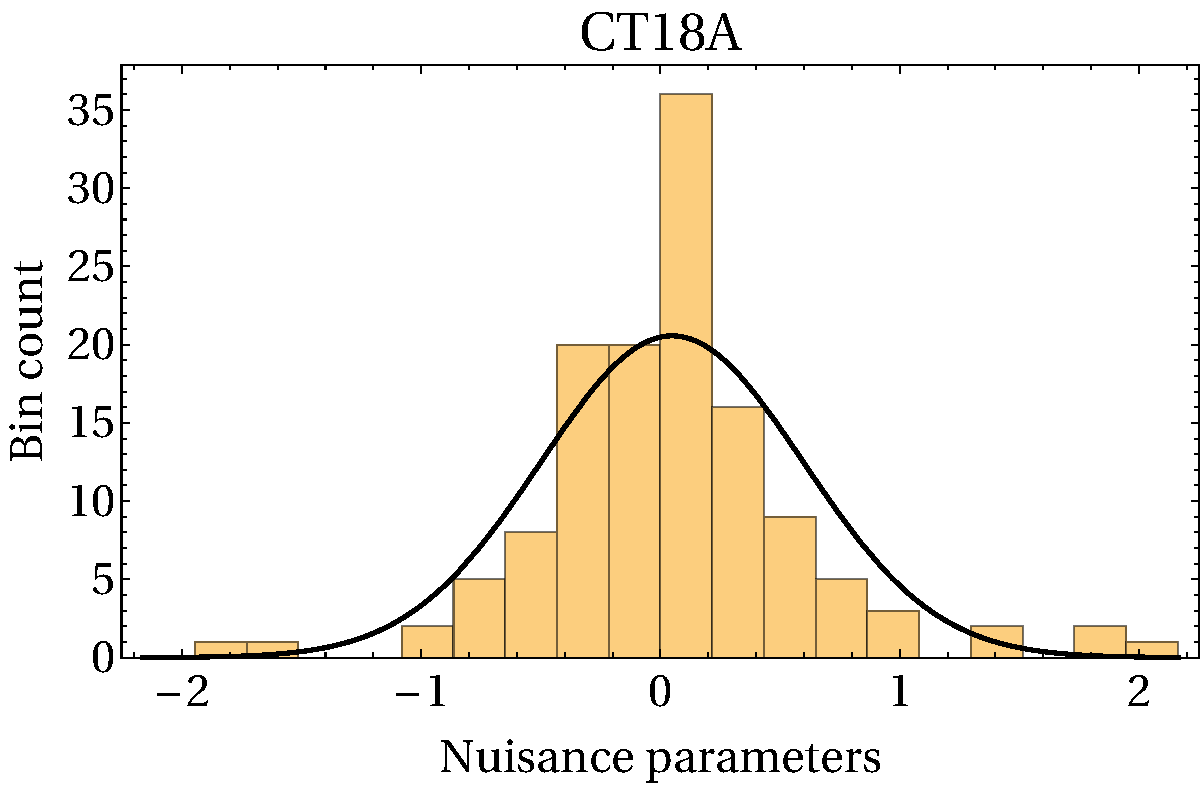
\includegraphics[width=0.44\textwidth]{fig/ATL7WZ/Nuisance_CT18A_ATL7WZ.pdf}\\
(a)\hspace{2in} (b)
	\caption{
		Histogram of (a) the shifted residuals and (b) nuisance parameters for the ATL7ZW data obtained for CT18A NNLO.
	}
\label{fig:248_hist}
\end{figure}

The $\chi^{2}_E/N_{pt,E}$ values for ATL7ZW data
quoted for the nominal NNPDF and MMHT fits are within the interval
covered by the candidate CT18 fits, given that the $\chi^2$ for this
data set can change drastically due to variations in $s(x,Q)$ caused
by minor adjustments in the fit's settings. The
nominal CT18A(Z) have a marginally higher $\chi^2_E/N_{pt,E}$ in
Table~\ref{tab:CMN} in part because 
NNPDF3.1 includes associated $W$-boson and charm-jet ($W+c$)
production from CMS at 7 TeV \cite{Chatrchyan:2013uja} in their
fit. When evaluated at NLO in QCD, as NNPDF has done using
MCFM \cite{Campbell:2010ff}, the $W+c$ data appear to prefer higher
$s(x,Q)$ values than the DIS experiments, especially the ATLAS $W+c$
measurement. While the positive pulls of ATL7ZW and $W+c$ data may add
up to increase $s(x,Q)$, we do not 
include $W+c$ measurements in CT18A(Z) yet because the full NNLO
calculation is still unavailable.
Neither are the NNLO massive heavy-quark
contributions for differential cross
sections of SIDIS dimuon production, needed to compute the detector acceptance when the fitted CCFR/NuTeV cross sections are reconstructed. 
The MMHT partial solution of further increasing the flexibility of the $s$ parametrization risks exacerbating the instabilities revealed by the LM scans or arriving at an incorrect Hessian uncertainty on $s(x,Q)$ that does not reflect the tension between the DIS and ATL7ZW experiments. We also point out non-negligible impacts of the differences between
the NNLO codes for ATL7ZW, cf. the end of Sec.~\ref{sec:Appendix4xFitter},
and of the NNLO QCD scale uncertainty,
with MMHT using $\mu_{R,F}=M_{W,Z}/2$ for ATL7ZW instead of 
$\mu_{R,F}=M_{W,Z}$ chosen for CT18A(Z).

\begin{figure}[tb]
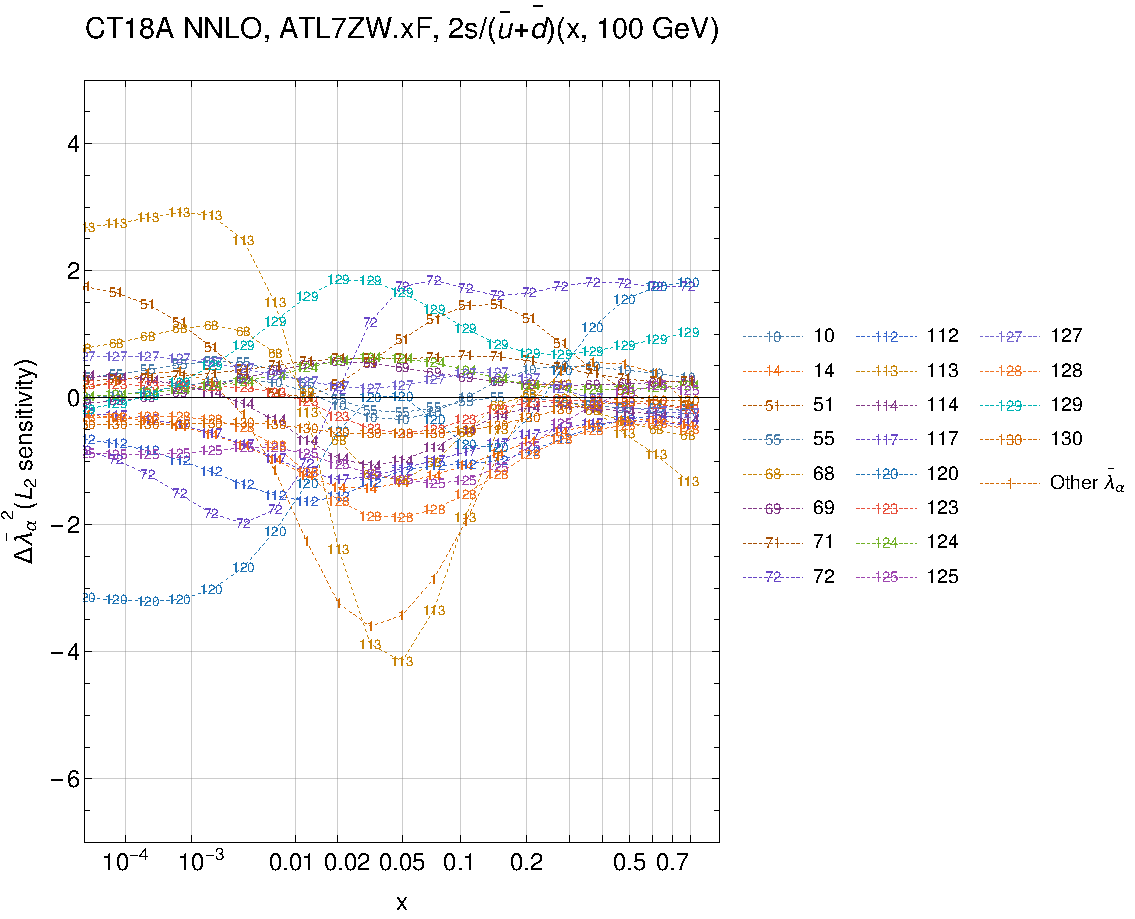
\includegraphics[width=0.9\textwidth]{fig/ATL7WZ/248rat_ifl5_lam_ct18Ann_lambda_q100.pdf}
	\caption{
		A plot, analogous to the $L_2$ sensitivity plots given above, showing the pulls of the correlated systematic uncertainties of the ATLAS $W/Z$ data
		on $R_s(x,Q=100\,\mathrm{GeV})$ in CT18A NNLO, as represented by shifts in the associated squared nuisance parameters, $\Delta \lambda^2_\alpha$.
	}
\label{fig:248_l2nui}
\end{figure}

\subsubsection{Comparisons to rapidity distributions}
\label{sec:ATL7ZWrap}

Figures~\ref{fig:248_DT}-\ref{fig:248_hist} show the theory-to-data
comparisons for CT18A/Z predictions against the ATL7ZW data set, the
distributions of shifted residuals in the final-state (pseudo)rapidity in
three individual channels, and the respective
cumulative histograms of the best-fit shifted
residuals $r_i$ and nuisance parameters $\bar\lambda_\alpha$.

In terms of the descriptions of the individual data points, the
figures indicate that CT18A/Z predictions describe $W^+$ production
well, while they show elevated differences with $W^-$ production
across the whole range of lepton pseudorapidities, as well with $Z$
production in the bins with the average $Z$-boson rapidity of 0.9 and 1.3.

Description of these data also require shifts of five nuisance
parameters $\bar \lambda_\alpha$,
labeled as 113, 72, 129, 125, and 128 in the ATLAS
data set, by $\approx \pm 2$ standard deviations. [These parameters
receive a mix of contributions from various systematic sources and
do not have a certain physics interpretation.]

A variation on the $L_2$ sensitivity technique allows us to demonstrate that
variations in these parameters are strongly linked to changes in the
strangeness ratio $R_s$ in the $x$ region probed by the ATL7ZW
measurement.
In the previous figures, the $L_2$ sensitivity approach explored the
connection between PDF variations and $\Delta \chi^2_E$
for individual experiments; but we can also compute
the $L_2$ correlation between the PDFs and contribution to $\chi^2$ from an individual nuisance parameter,  
$\Delta \bar \lambda^2_\alpha(a)$ 
for $\alpha=1,...,\ N_\lambda$, contributing to $\Delta \chi^2_E(a)$ according to Eq.~(\ref{Chi2a0l0}) for arbitrary $a\approx a_0$. In Fig.~\ref{fig:248_l2nui}, we demonstrate this for the ATL7ZW data, showing the
pulls of the ATL7WZ correlated systematic uncertainties on $R_s$ at $Q=100$ GeV in CT18A. While most nuisance parameter shifts
stay within $|\Delta \lambda^2_\alpha|\! \sim\! 1\!-\!2$ units, a
small collection of $\bar \lambda_\alpha$
are strongly sensitive to the fitted $R_s$ at various $x$,
notably parameters 113, 72, 120, and 129,
%
{\color{red} (TIM) of which
some very nearly approach (parameters 72 and 129) or exceed (parameters 113 and 120)
the bound of $|\Delta \lambda^2_\alpha|\! <\!2$.
}

While we do not have information to reveal the specific causes driving
these systematic sources, it is clear that some have profound
effect on the preferred $R_s$ behavior in the intervals of $x$ that
can be read off Fig.~\ref{fig:248_l2nui}.

% ~ ~ ~ ~ ~ ~ ~ ~ ~ ~ ~ ~ ~ ~ ~ ~ ~ ~ ~ ~ ~
% ~ ~ ~ ~ ~ ~ ~ ~ ~ ~ ~ ~ ~ ~ ~ ~ ~ ~ ~ ~ ~ 

\subsection{Scans on PDFs, $\alpha_s$, and $m_c$ in CT18Z
\label{sec:LMCT18Z}
}

We conclude this Appendix with a few results from Lagrange Multiplier
scans, the powerful technique applied at the end of the global
analysis cycle to obtain a close look at the exact probability
distributions that cannot be gleaned from the fast, but approximate,
Hessian studies. The results presented here for CT18Z NNLO
complement an analogous discussion for CT18
presented in Sec.~\ref{sec:QualityOverview}. By examining the
$\Delta \chi^2$ values that are returned from the full
fit rather than from the fast linearized approximations,
we discover subtle features such as the tensions
among experiments or instability/multiple solutions of the fit for
some PDF combinations. 
%
%

\begin{figure}[htbp]
\begin{center}
	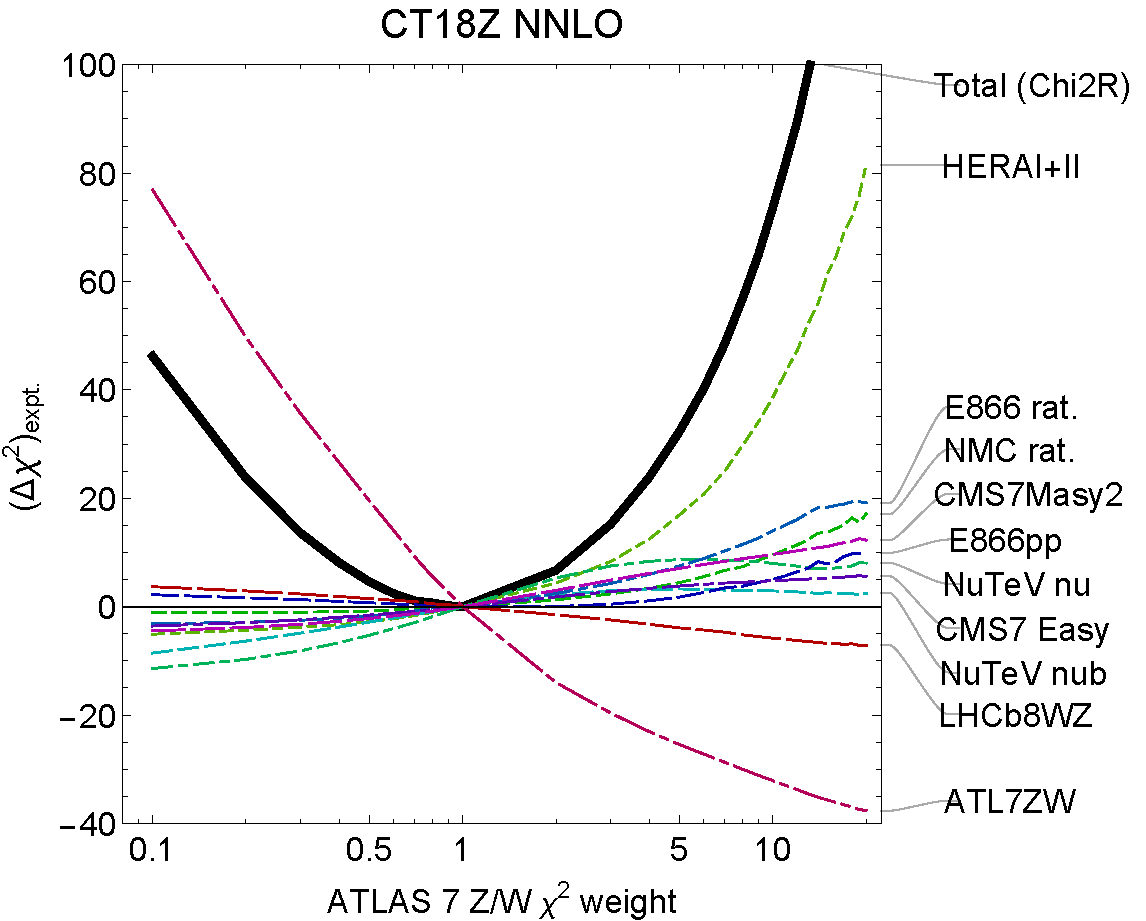
\includegraphics[width=0.48\textwidth]{./fig/ATL7ZWWT_scan2Tct18z.pdf}\quad
	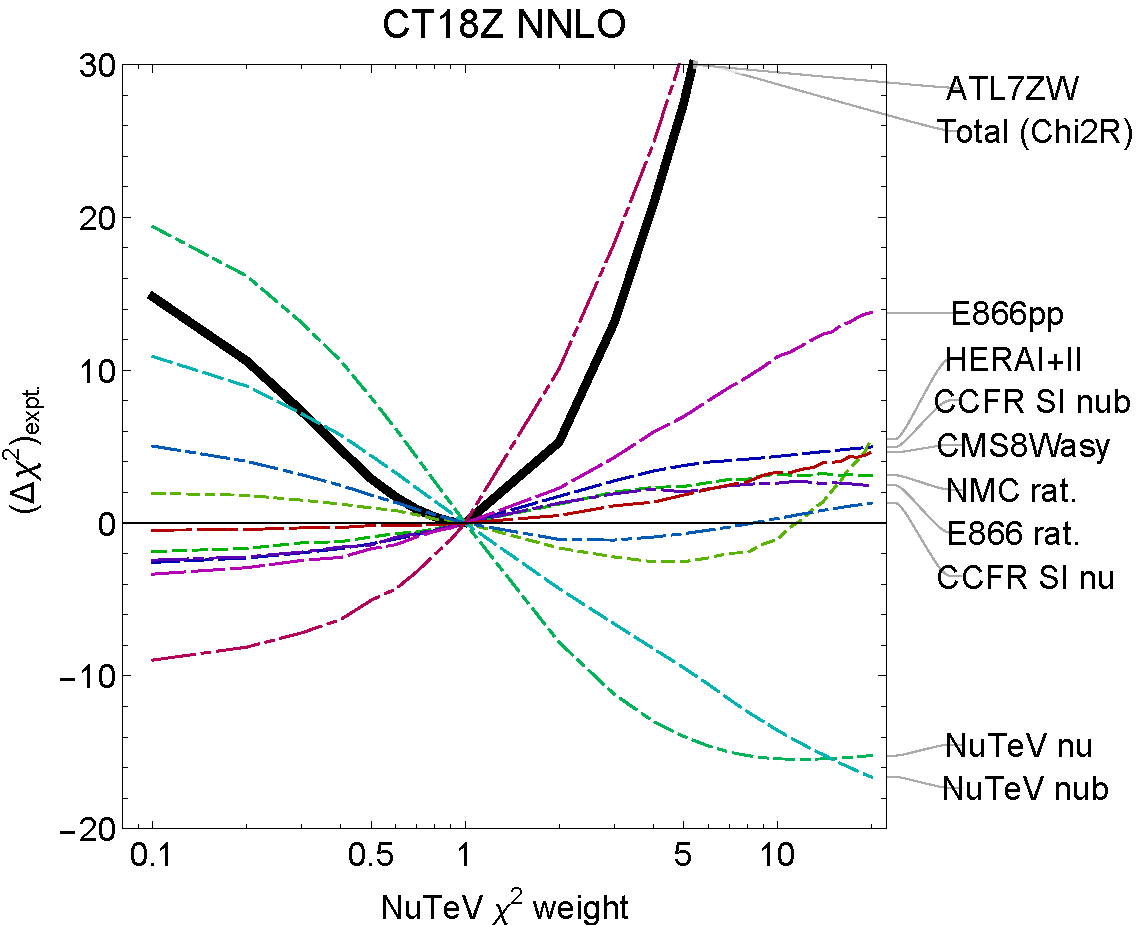
\includegraphics[width=0.48\textwidth]{./fig/NuTeVWT_scan2Tct18z.pdf}
	\caption{(Left panel) The change in total $\chi^2$, $\Delta \chi^2$, of the leading data sets included in the CT18Z NNLO fit
	when varying the weight of the ATL7ZW data away from weight $w\!=\!1$ as in the default fit. (Right panel)
	The analogous plot for the NuTeV $\nu,\, \bar{\nu}$ SIDIS dimuon data (Exp.~IDs=124, 125).
	}
\label{fig:lm_wht}
\end{center}
\end{figure}

\subsubsection{Scans with varied statistical weights of ATLAS 7 TeV $W/Z$ and NuTeV data}
\label{sec:ATL7ZWchi2wt}

The evident tension between the ATL7ZW data and other experiments can
be examined in terms of the variation of $\chi^2_E$ for a number of 
most sensitive experiments, when the weight of the ATL7ZW data is varied
within the CT18Z NNLO fit \cite{Collins:2001es}.  
The results of this are shown in the left panel of
Fig.~\ref{fig:lm_wht}, in which the weight of the ATL7ZW data is
continuously tuned from $w\!=\!0.1$ (sharply de-emphasizing this information, shifting $\chi^2_E$ by $\Delta \chi^2_E\! \sim\! +80$)
to $w\!=\!20$ (strongly over-weighting the ATLAS data, leading to a
$\Delta \chi^2_E\! \sim\! -40$ improvement in their description in CT18Z). 

The figure also shows the curves for the experiments with the largest
variations in their $\Delta \chi^2_E$ when the $\chi^2$ weight of the
ATL7ZW data set is changed. 
A notable feature to observe in the left inset
is that it is the combined HERAI+II
inclusive DIS data set (Exp.~ID=160), rather than other experiments, that mostly
opposes including the ATL7ZW data set with a weight of 5-10.
With the exception of the LHCb 8 TeV $W/Z$
data (250), which is described better when the weight of ATL7ZW
is increased, the rest of the plotted experiments oppose such increase.
These experiments include E866 (203) and NMC (104) $p/d$ ratio,
NuTeV dimuon production (124, 125), and CMS 7 TeV $\mu$- and $e$-asymmetries
data (266 and 267).

As the ATLAS data are deemphasized ($w\!\sim\!0.1$),
the descriptions of the NuTeV SIDIS
dimuon-production data sets (Exp.~IDs=124, 125) are most improved,
further suggesting some tension.

These observations are consistent with the companion scan shown in
the right inset, which
similarly plots the $\Delta \chi^2$ variations of the experiments most
responsive to changing the weight of the NuTeV dimuon data.
Especially considering $N_{pt}$ for the plotted
experiments, the heavy over-weighing of the NuTeV data
leads to a very rapid deterioration of $\chi^2$ for the ATL7ZW points,
which in fact worsens more quickly than the full
CT18Z global analysis as the NuTeV weight is increased.
In fact, the $\chi^2_E$ for the inclusive HERA (160) and CCFR neutrino
dimuon production (126) mildly improves when the NuTeV weight is
increased to about 5. On the other hand, E866 $pp$ (204), CCFR
antineutrino dimuon (127), CMS 8 TeV charge asymmetry (249), and NMC $pd$
ratio (104) oppose such increase. 

%
\begin{figure}[htbp]
\begin{center}
	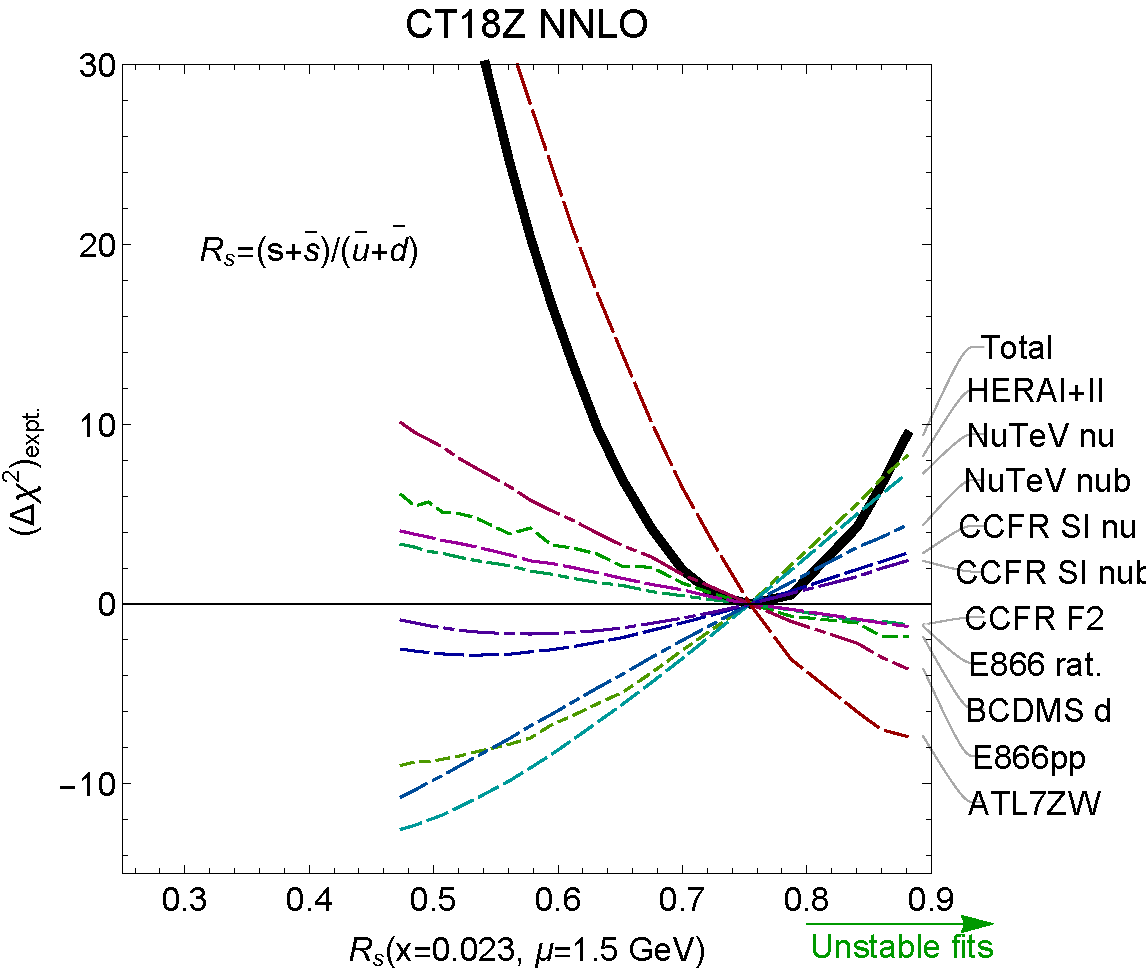
\includegraphics[width=0.48\textwidth]{./fig/Rs_scan2Tct18z_1.pdf}\quad
	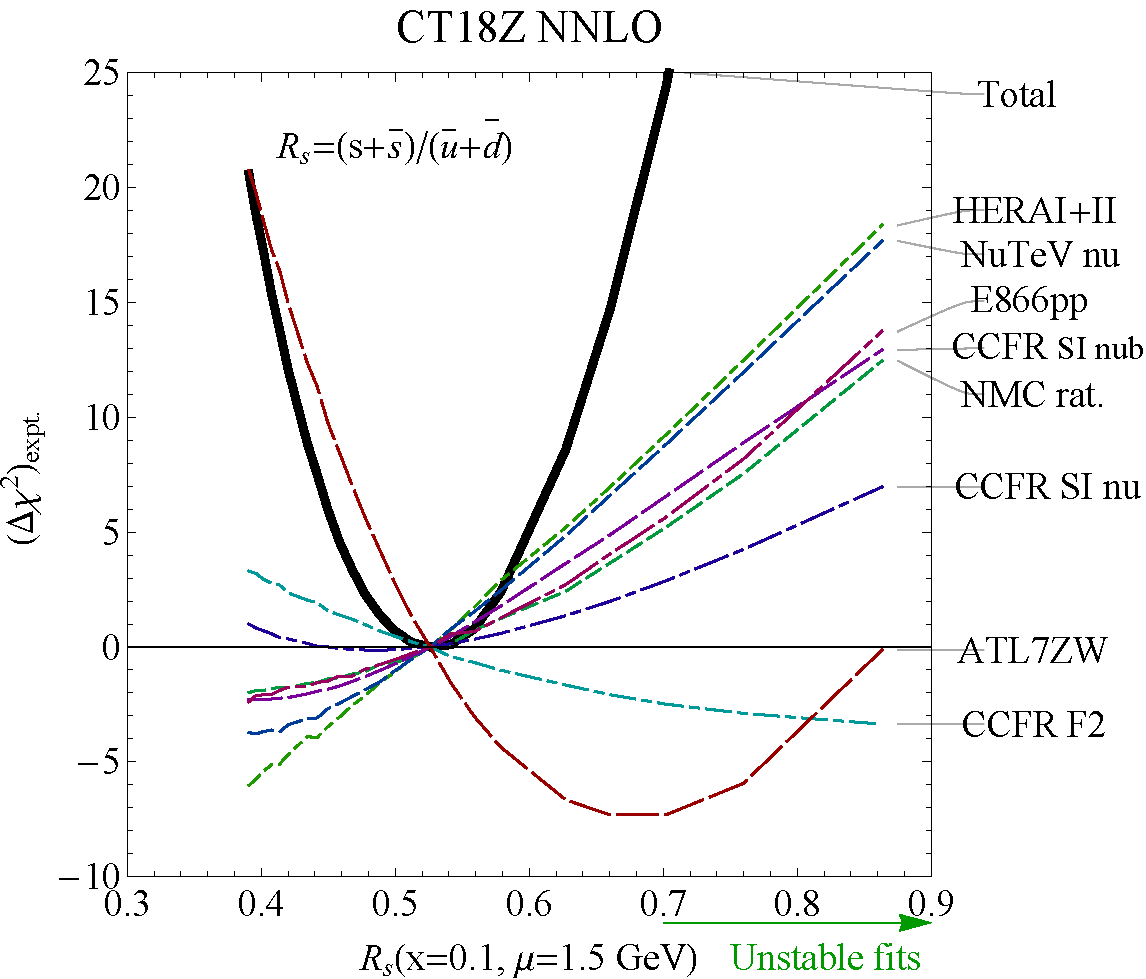
\includegraphics[width=0.48\textwidth]{./fig/Rs_scan2Tct18z_2.pdf}\\
(a)\hspace{2.6in}(b)\\
	\caption{The Lagrange Multiplier scan of $R_s$ at $Q=1.5$ GeV, $x=0.023$ and $x=0.1$ for the (a,b) CT18Z fit, analogous to Fig.~\ref{fig:LMRs} for CT18.
\label{fig:lm_rsz}}
\end{center}
\end{figure}
%


\subsubsection{LM scans on the strangeness ratio $R_s$ for CT18Z}
\label{sec:LMRsCT18Z}

%
%
\begin{figure}[htbp]
\centering
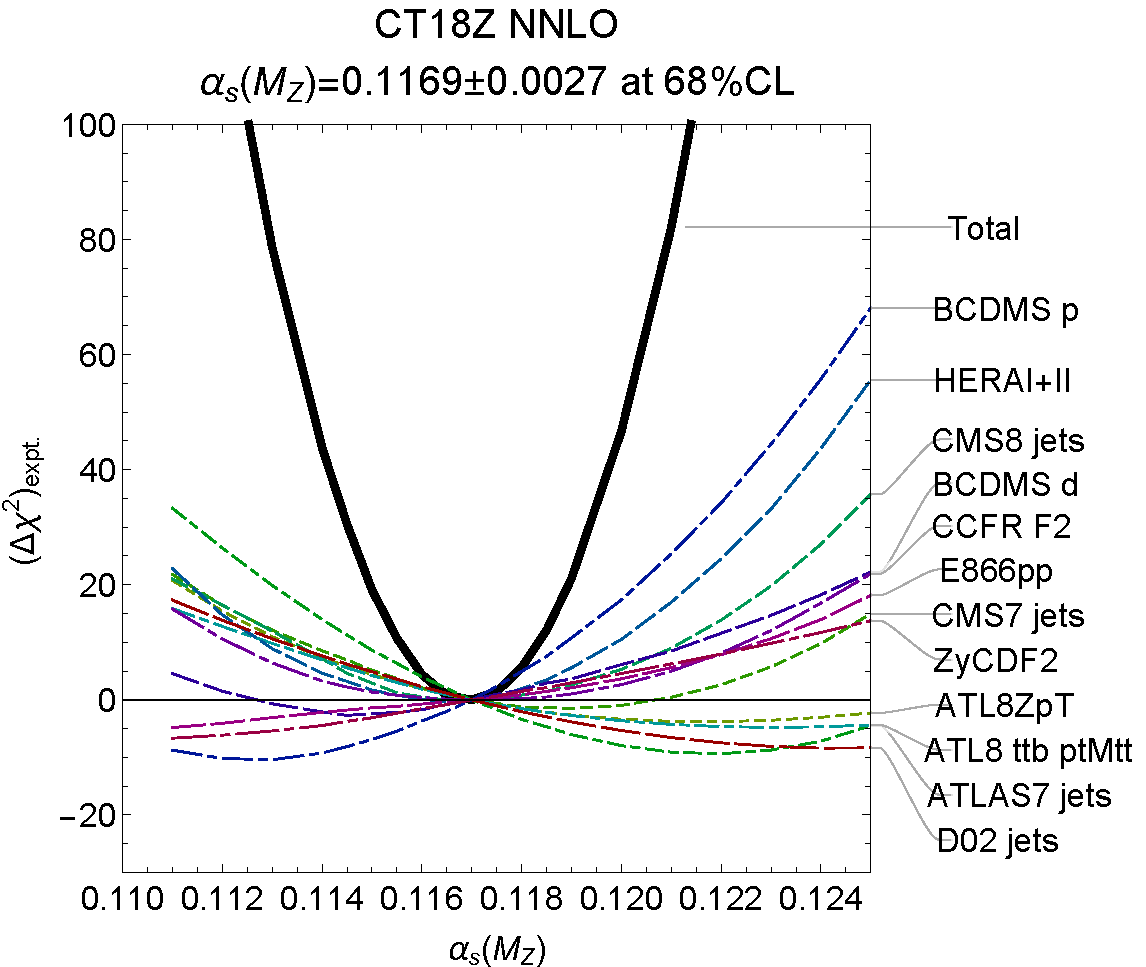
\includegraphics[width=0.49\textwidth]{./fig/alphas_scanTct18z_pjb05b.pdf}\quad
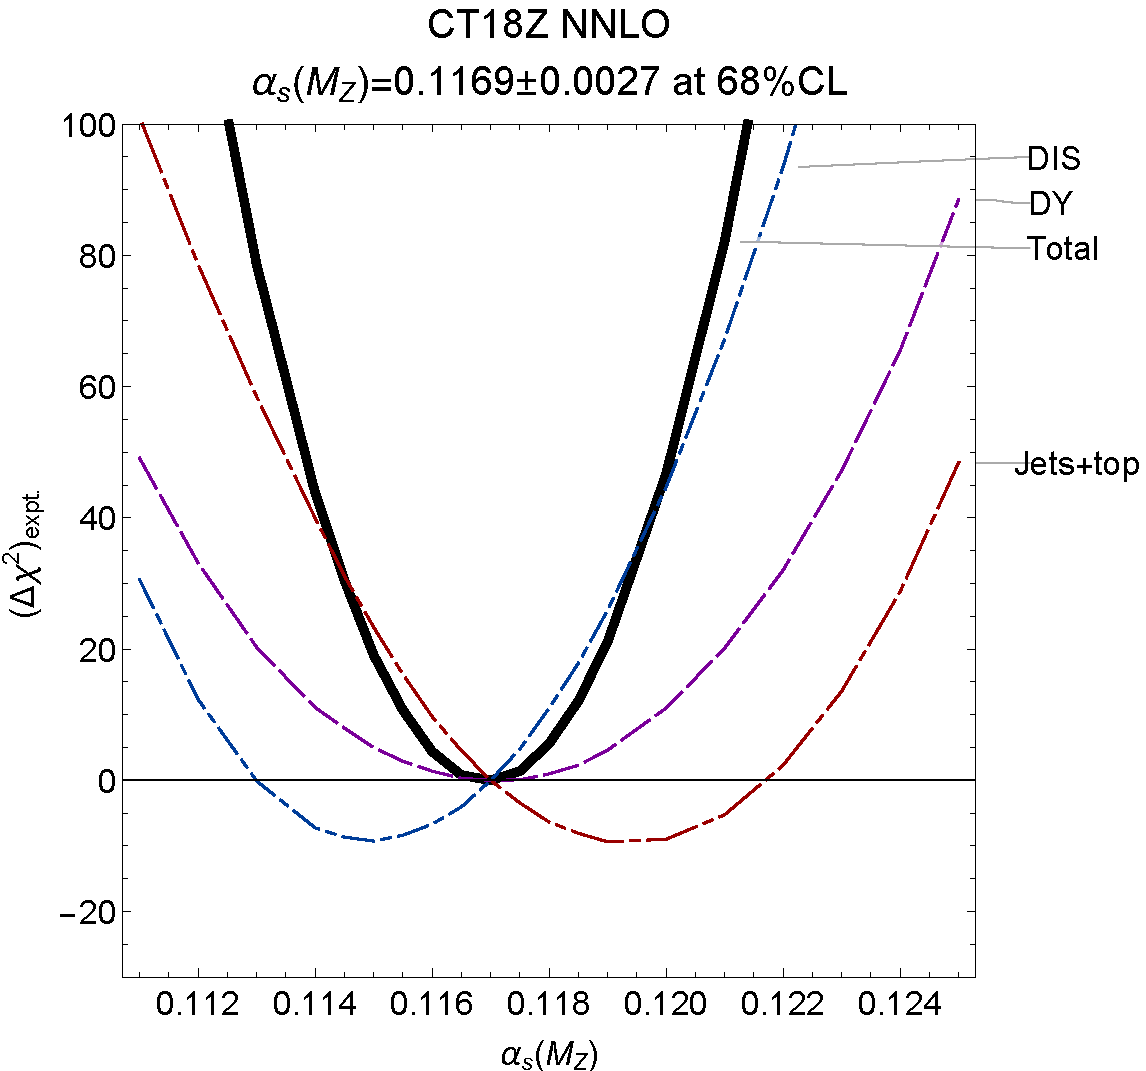
\includegraphics[width=0.46\textwidth]{./fig/alphas_scanTct18z_pjb05b2.pdf}\quad
\caption{Scans over the strong coupling at the scale of $M_Z$ for CT18Z,
	analogous to Fig.~\ref{fig:lm_alphas} for CT18. As before, we show in the left panel
	the $\Delta \chi^2$ variations for a number of experiments with leading sensitivity
	to $\alpha_s(M_Z)$, while the right panel again shows the change in $\chi^2$ for all experiments
    fitted in CT18Z, separately collected into combined DIS, DY and top/jets data sets. Also as before,
    the ``Jets+top'' curve in the right panel is primarily influenced by the jet production data sets. Due to the
    intermediate impact of the $t\bar{t}$ data noted in Fig.~\ref{fig:lm_alphas}, variations in the
    CT18 fit leading to CT18Z are such that the ATLAS 8 TeV $t\bar{t}$ data (Exp.~ID=580) are now
    selected with the ensemble of sensitive experiments in the left panel.
\label{fig:lm_alphasz}}
\end{figure}

Lagrange Multiplier scans on the strangeness ratio $R_s(x,Q)$, shown
for CT18Z NNLO in Fig.~\ref{fig:lm_rsz} at $Q\!=\!1.5$ GeV and two
representative momentum fractions, 
$x\!=\!0.023$ (in the left panel) and $x\!=\!0.1$ (in the right),
reveal several important features that are also observed in the other
LM scans we have performed. 

\begin{enumerate}

\item Both panels of Fig.~\ref{fig:lm_rsz} reveal the opposing preferences
of, {\it e.g.}, the HERA DIS and NuTeV/CCFR SIDIS sets for a smaller value of
$R_s$, peaked more toward $R_s\!\sim\! 0.5$ at both values of $x$,
and the positive pull of the ATL7ZW data, supported by weaker pulls of
E866 $pd$ ratio (203), BCDMS $F_2^d$ (102), and especially
$F_2$ CCFR neutrino (110) data, which is very pronounced at $x=0.1$.

\item When $R_s$ is forced to take values above 0.7-0.8, the $\chi^2$
starts to fluctuate irregularly in both scans and fails to converge in
many fits as $R_s$ is pushed to even higher values.

\item In reflection of the above strong trade-off between the pulls of the
DIS and ATL7ZW data sets, we observe that the Hessian uncertainty
based on the dynamic tolerance similar to the one used by MMHT reports
a narrower uncertainty on $R_s(x,Q)$ than seems reasonable to expect based on the $\chi^2$ contributions of individual experiments.

\end{enumerate}

\subsubsection{CT18 LM scans on $\alpha_s(M_Z)$ and $m_c$}
\label{sec:CT18Zalphas}
%
The various modifications in CT18Z, especially the use of the
$x_B$-dependent scale $\mu_{F,x}$ in DIS experiments that provide the
largest coverage in the energy scale $Q$, modify 
the constraints on the strong coupling, $\alpha_s(M_Z)$,
for which we plot the scans in Fig.~\ref{fig:lm_alphasz}.
%

%
\begin{figure}[htbp]
\centering
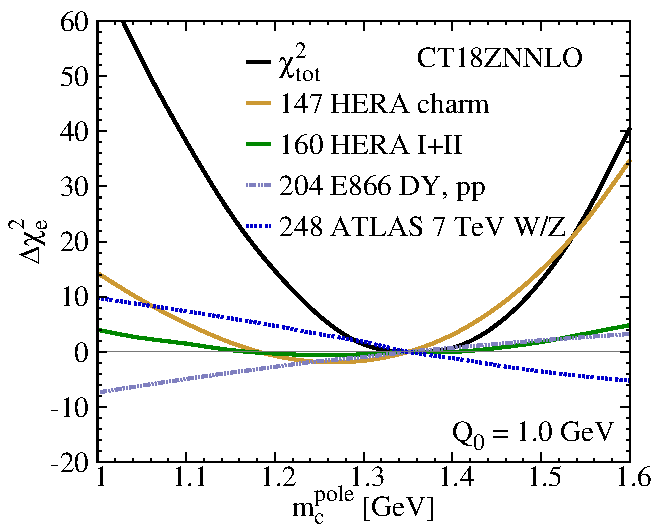
\includegraphics[width=0.6\textwidth]{./fig/LM/i2TZn3Q01-00mc1-35_DEchi2_re_ect.pdf}
\caption{
        Analogously to Fig.~\ref{fig:lm_mc}, the scan over values of the charm pole mass, $m_c$, computed here using CT18Z NNLO following the procedure described in Sec.~\ref{sec:AlphasDependence}. 
        }
\label{fig:lm_mcZ}
\end{figure}
%

Although the $68\%$ C.L.~determination of $\alpha_s(M_Z)\! =\!
0.1169\! \pm\! 0.0027$ agrees closely with the CT18-based
determination (with the latter being only slightly weaker and with an
identical uncertainty), the experimental pulls have notable
differences. Most strikingly, there is a separation in the preferences
of the combined inclusive jet-production data and Drell-Yan experiments,
which were aligned closely for CT18 in Fig.~\ref{fig:lm_mc}. The
combined Drell-Yan data (including ATL7ZW) now agree very closely with
the preferred value of the full CT18Z fit, but the DIS and
jet+$t\bar{t}$ data pull $\alpha_s(M_Z)$ in the opposite directions
more strongly than in CT18.

Such visible dependence of the preferred ranges for $\alpha_s(M_Z)$
from three categories of experiments on the DIS QCD scale may
indicate presence of important uncertainties beyond NNLO that are not
accounted in the nominal 68\% C.L. uncertainty of 0.0027.

%
Similarly, the choices made in the alternative CT18X/A/Z global
analyses can lead to different preferences in these fits for the
charm pole mass, $m_c^{pole}$.
While we described the $m_c$ scan in detail 
in the case of CT18 in Sec.~\ref{sec:AlphasDependence},
repeating this scan for CT18Z NNLO leads to a somewhat different
behavior shown in Fig.~\ref{fig:lm_mcZ}.
Although CT18Z ultimately arrives at a very similar central value of
$m_c$, the interplay of sensitive
experiments now is somewhat different than that
shown for CT18 in Fig.~\ref{fig:lm_mc}.
The pull of the combined HERA data (160) on $m_c$
decreases in CT18Z, the preferred $m_c$
of the HERA charm-production data (Exp.~ID=147)
increases slightly. In addition, the ATL7ZW data
also exhibit a modest preference for larger charm masses, and
these latter two experiments produce a small increase in the
central preferred value of $m_c$ in CT18Z relative to CT18,
although with a similar extent of uncertainty.


%-  -  -  -  -  -  -  -  -  -  -  -  -  -  -  -  -  -  -  -  -  -  -  -  -  -  -  -  -  -  -  -  -  -
\clearpage

\section{CT18 goodness-of-fit function and treatment of correlated uncertainties}
\label{sec:chi2_app}
%
%
\newcommand{\betamat}{b}

In this appendix, we summarize the implementation of the
goodness-of-fit function $\chi^2$ and marginalization of nuisance
parameters in the CT18 family of fits. For the latter task, we
normally follow a procedure, adopted since the CTEQ6 analysis, to
estimate the correlated uncertainties using the correlation matrix
published by the experiment. For the few data sets that do not provide
the correlation matrix, we find it convenient to present the
covariance matrix in an approximate form that separates the
uncorrelated and correlated components. The algorithm for this
conversion is explained at the end of the appendix.   


{\bf Definitions.}
%
In Eq.~(\ref{Chi2sys}) of Sec.~\ref{sec:chi2}, we introduced the standard
goodness-of-fit function $\chi^{2}$ used in the recent CT fits. Here
we review its treatment using a matrix notation.

%
We express $D_{k},$ $T_{k},$ and $\beta_{k\alpha}$
in units of $s_{k}$ for each $k$. That is, we introduce a vector
$d\equiv S^{-1}\left(D-T(a)\right)$ of length $N_{pt}$, where
\begin{equation}
S\equiv\mbox{diag}\left\{ s_{1},s_{2},...,s_{N_{pt}}\right\} .\label{S}
\end{equation}
Similarly, $\lambda\equiv\{\lambda_{\alpha}\}$ is a vector of length
$N_{\lambda}$; and $\betamat\equiv S^{-1}\beta$ is a rectangular matrix
of dimension $N_{pt}\times N_{\lambda}$.
%
In this matrix notation, Eq.~(\ref{Chi2sys}) takes the form
\begin{equation}
\chi_{E}^{2}(a,\lambda)=\left(d-\betamat\lambda\right)^{T}(d-
\betamat\lambda)+\lambda^{T}\lambda.\label{Chi2sys2}
\end{equation}

{\bf Minimization of $\chi^{2}$.}
%
The solution for the minimal value of $\chi^{2}$ (with respect to nuisance parameters) is found in terms
of the following matrices:
\begin{align}
\mathcal{A}\equiv\mathcal{I}+ {\betamat}^{T}\betamat;~~~ & C\equiv I+\betamat\betamat^{T};\label{ACm1}\\
\mathcal{A}^{-1}=\mathcal{I}-\betamat^{T}C^{-1}\betamat;~~~ & C^{-1}=I-\betamat\mathcal{A}^{-1}\betamat^{T}.\label{Am1C}
\end{align}
Uppercase roman and script letters denote matrices of dimensions $N_{pt}\times N_{pt}$
and $N_{\lambda}\times N_{\lambda}$, respectively. Therefore, $I$
is an $N_{pt}\times N_{pt}$ identity matrix, and $\mathcal{I}$ is
an $N_{\lambda}\times N_{\lambda}$ identity matrix. $C$ and $\mathcal{A}$
are covariance matrices (appropriately normalized by $s_{k}$) in
spaces of data values and nuisance parameters, respectively. The relations
between ${\cal A}^{-1}$ and $C^{-1}$ in Eq.~(\ref{Am1C}) can be
demonstrated by using $\betamat^{T}\betamat=\mathcal{A}-\mathcal{I}$ and
$\betamat\betamat^{T}=C-I$. The covariance matrices are symmetric: $\mathcal{A}^{T}=\mathcal{A},$
$C^{T}=C$.

For each theory input $a$, $\chi^{2}$ can be minimized with respect
to $\lambda$ analytically, by solving for $\partial\chi^{2}/\partial\lambda_{\alpha}=0$
\cite{Pumplin:2002vw}. The solution is
\begin{align}
 & \bar{\lambda}(a)=\mathcal{A}^{-1}\betamat^{T}d=\betamat^{T}C^{-1}d;\label{lambda0}\\
 & \bar{\lambda}^{T}(a)=d^{T}\betamat\mathcal{A}^{-1}=d^{T}C^{-1}\betamat.
\end{align}
 The global minimum $\chi^{2}(a_{0},\lambda_{0})$ for all experiments
$E$ can be found numerically as
\begin{equation}
\chi^{2}(a_{0},\lambda_{0})=\sum_{E}\ d_{0}^{T}C^{-1}d_{0},\label{Chi2CovMat}
\end{equation}
 with $d_{0}\equiv S^{-1}\left(D-T(a_{0})\right)$, $\lambda_{0}\equiv\bar{\lambda}(a_{0})$.

An equivalent form of this equation can be derived,
\begin{equation}
\chi^{2}(a_{0},\lambda_{0})=\sum_{E}\ \left(r_{0}^{T}r_{0}+\lambda_{0}^{T}\lambda_{0}\right),\label{Chi20rl}
\end{equation}
where $r_{0}$ are the best-fit shifted residuals:
\begin{equation}
r_{0}\equiv S^{-1}\left(d_{0}-\betamat\lambda_{0}\right)=\bar{r}(d_{0}),\mbox{~with~}\bar{r}(d)\equiv C^{-1}d.\label{r0}
\end{equation}
The representation (\ref{Chi20rl}) is particularly informative. We
anticipate that, in a good fit of theory to an experiment $E$, the
shifted residuals $r_{0}$, quantifying agreement with individual
data points, as well as the nuisance parameters $\bar{\lambda}_{0}$,
quantifying the systematic shifts, are distributed according to their
own standard normal distributions, ${\cal N}(0,1)$. Comparisons of
the two empirical distributions to the expected ${\cal N}(0,1)$ distributions
serve as the tests for the goodness of fit and for the implementation
of systematic errors \cite{Kovarik:2019xvh}.

{\bf Decomposition of the covariance matrix.}
%
%
The form of $\chi^2$ in Eq.~(\ref{Chi2CovMat1}) coincides with Eq.~(\ref{Chi2CovMat}),
obtained by optimizing the nuisance parameters $\lambda$ for a given $a$, in the prevalent
case when we separately know the uncorrelated and fully correlated
systematic errors. In this case, we identify
\begin{equation}
\mbox{cov}=SCS,~~~\mbox{cov}^{-1}=S^{-1}C^{-1}S^{-1}.\label{SCS}
\end{equation}
 The matrix elements, according to Eqs.~(\ref{ACm1}) and (\ref{Am1C}),
are
\begin{align}
\left(\mbox{cov}\right)_{ij} & =s_{i}^{2}\delta_{ij}+\sum_{\alpha=1}^{N_{\lambda}}\beta_{i\alpha}\beta_{j\alpha},\label{cov}\\
\left(\mbox{\mbox{cov}}^{-1}\right)_{ij} & =\frac{\delta_{ij}}{s_{i}^{2}}-\sum_{\alpha_1,\alpha_2=1}^{N_{\lambda}}\frac{\beta_{i\alpha_1}}{s_{i}^{2}}{\cal {\cal A}}_{\alpha_1\alpha_2}^{-1}\frac{\beta_{j\alpha_2}}{s_{j}^{2}}.\label{covm1}
\end{align}
In particular, a diagonal element $(\mbox{cov})_{ii}$ {[}no summation{]}
is the quadrature sum of the statistical, uncorrelated systematic,
and correlated systematic uncertainties:
\begin{equation}
(\mbox{cov})_{ii}=s_{i,\mbox{\scriptsize stat}}^{2}+s_{i,\mbox{\scriptsize uncor sys}}^{2}+s_{i,\mbox{\scriptsize cor sys}}^{2},\label{s2i}
\end{equation}
where $s_{i,\mbox{\scriptsize cor sys}}^{2}\equiv\sum_{\alpha}\beta_{i\alpha}^{2}$.
With the help of Eq.~(\ref{SCS}), the shifted residuals in Eq.~(\ref{r0})
then are written as
\begin{equation}
r_{i}\equiv\frac{D_{i}^{sh}(a)-T_{i}(a)}{s_{i}}=s_{i}\sum_{j=1}^{N_{pt}}\left(\mbox{\mbox{cov}}^{-1}\right)_{ij}\left(D_{i}-T_{i}(a)\right).\label{ricov}
\end{equation}
Computing them thus requires that we know the full uncorrelated error $s_{i}=\sqrt{s_{i,\mbox{\scriptsize stat}}^{2}+s_{i,\mbox{\scriptsize uncor sys}}^{2}}$.

{\bf Finding a correlation matrix from the covariance matrix.} In some experimental measurements, such as the LHCb 8 TeV W/Z production \cite{Aaij:2015zlq},
only the full covariance matrix is provided, making impossible the straightforward
reconstruction of the shifted residuals according to Eq.~(\ref{ricov}).
%For instance, it may happen that some systematic parameters $\lambda$ are
%not independent (are partly correlated). We can still perform a number
%of instructive comparisons of the theory with the individual data for
%such an experiment.
%
%\begin{enumerate}
%\item We can estimate the shifted residuals $r_{i}$ in Eq.~(\ref{ricov})
%assuming full correlation of systematic effects, i.e., setting $s_{i,\mbox{\scriptsize uncor sys}}=0$
%and $s_{i}=s_{i,\mbox{\scriptsize stat}}.$ This estimate presents
%a lower bound on a shifted data point residual under an arbitrary
%degree of correlation.
%\item We can diagonalize the inverse covariance matrix for experiment $E$,
%\begin{equation}
%\text{cov}^{-1}=OR^{T}RO^{T},~~,O^{T}=O^{-1},~~\chi_{E}^{2}(\{a_{0}\})=\sum_{l=1}^{N_{pt}}R_{l}^{2},
%\end{equation}
%and compare the diagonalized residuals
%\begin{equation}
%R_{l}\equiv\sum_{j,k=1}^{N_{pt}}R_{lj}O_{jk}\left(D_{k}-T_{k}(\{a_{0}\})\right).
%\end{equation}
%The data point residuals with a high degree of correlation will be
%mixed by this ortogonal transformation.
%\item 
In several cases, we find it feasible to iteratively reconstruct the
approximate uncorrelated systematic and correlated systematic contributions,
$s_{k,\mbox{\scriptsize uncor sys}}$ and $\beta_{k\alpha}$, from the
provided covariance matrix $\mbox{cov}\equiv K_{0}$, by assuming
that the systematic shifts are dominated by a certain number $M_{\lambda}$,
with $M_{\lambda}\leq N_{\lambda}$, of fully correlated linear combinations.
The approximation makes use of the positive-definiteness of the covariance
matrix and its diagonal elements, cf.~Eq.~(\ref{s2i}). It represents
the original covariance matrix by a numerically close matrix
given by the sum of a diagonal matrix $\Sigma$, interpreted as consisting of total uncorrelated errors, and a non-diagonal square matrix $K$, interpreted as a product of the correlation matrix $\beta$ and its transpose.

In particular,
suppose we find the eigenvalues $x_{k}^{2}$ of $K_{0}$ and sort
them in the descending order:
\begin{align}
K_{0} & =O^{T}xO,\mbox{ with }x=\mbox{diag}\left\{ x_{1}^{2},x_{2}^{2},...,x_{N_{pt}}^{2}\right\} ,\label{K0}\\
 & x_{1}^{2}\geq x_{2}^{2}\geq...\geq x_{N_{pt}}^{2}>0.
\end{align}
Here $O$ is an orthogonal matrix.
We partition $x$ into a matrix $y$ containing the largest $M_{\lambda}$
eigenvalues and a matrix $z$ with the smallest ($N_{pt}-M_{\lambda})$
ones:
\begin{align}
y & \equiv\mbox{diag}\left\{ x_{1}^{2},x_{2}^{2},...,x_{M_{\lambda}}^{2},0,...,0\right\} ,\\
z & \equiv\mbox{diag}\left\{ 0,...,x_{M_{\lambda+1}}^{2},...,x_{N_{pt}}^{2}\right\} .\label{z}
\end{align}
Recalling that the diagonal elements of matrices $Y=O^{T}yO$ and
$Z=O^{T}zO$ are non-negative, we then construct a diagonal matrix
$\Sigma_{1}\equiv\mbox{diag}\left\{ Z_{11},...,Z_{N_{pt}N_{pt}}\right\} $
with $Z_{ii}>0,$ and another positive-definite matrix, $K_{1}\equiv Y+Z-\Sigma_{1}.$
We can iterate the steps in Eqs.~(\ref{K0})-(\ref{z}) by computing
$\Sigma_{a+1}$ and $K_{a+1}$ at step $a$ as
\begin{align}
\Sigma_{a+1} & \equiv\Sigma_{a}+\mbox{diag}\left\{ Z_{11},...,Z_{N_{pt}N_{pt}}\right\} ,\\
K_{a+1} & \equiv Y+Z-\mbox{diag}\left\{ Z_{11},...,Z_{N_{pt}N_{pt}}\right\} .
\end{align}
Here the matrices $Y$ and $Z$ are recomputed in each step using $K_{a}$ as the
input. After a sufficient number of steps $a$, the sum
\begin{equation}
C_{a}\equiv\Sigma_{a}+Y_{a}\label{Ca}
\end{equation}
approaches an asymptotic matrix that is close to the input matrix
$K_{0}$ in the sense of the $L_{p}$ norm $\sum_{i,j=1}^{N_{pt}}\left|(K_{0})_{ij}-(C_{a})_{ij}\right|^{p}$
with $p=2$ or $1$. If the extraction of the uncorrelated and fully
correlated components is feasible, the asymptotic $L_{p}$ distance
can be made small by choosing a large enough $M_{\lambda}$. For the
three experiments \cite{Aaij:2015gna,Aaij:2015zlq,Khachatryan:2016pev} in the CT18 data set that provide only the covariance
matrices, the $M_\lambda$ values giving good convergence
lie in the range between $N_{\lambda}/2$ and $N_{\lambda}$. 

By comparing
Eqs.~(\ref{cov}) and (\ref{Ca}), we identify
\begin{align}
(\Sigma_{a})_{ij} & \approx s_{i}^{2}\delta_{ij},\\
(Y_{a})_{ij} & \approx\sum_{\alpha=1}^{M_{\lambda}}\beta_{i\alpha}\beta_{j\alpha}.
\end{align}
Hence, $s_i$ is estimated from $(\Sigma_a)_{ij}$; and $\beta_{i\alpha}$ can be estimated from $(Y_{a})_{ij}$ by singular
values decomposition.
%\end{enumerate}


\section{Non-perturbative parametrization forms}
\label{sec:AppendixParam}
%
%
%
As noted in Sec.~\ref{sec:Paramstudies}, to obtain realistic estimates of the parametric PDF uncertainties, the CT global analyses explore a broad range of parametric forms for the PDFs at the starting scale, $Q\! =\! Q_0$. The goals
of these investigations are ({\bf i}) to select a sufficiently flexible functional form capable of fitting an
expansive high-energy data set without overfitting; and ({\bf ii}) to understand the uncertainties 
associated with the choice of parametrization.

% ' 2dvl'   981  0.1344059  0.0000000   0.76650   3.03816   2.64013   1.82667   2.73045   0.00000   0.00000   0.00000   0.00000   0.00000   0.00000   0.00000
% ' 1uvl'   981  0.3254043  0.0000000   0.76650   3.03816   1.50813  -0.13530   1.67016   0.00000   0.00000   0.00000   0.00000   0.00000   0.00000   0.00000
% ' 0glu'   848  0.3843830  0.0000000   0.53015   3.15246   3.03283  -1.70197   0.00000   0.00000   0.00000   0.00000   0.00000   0.00000   0.00000   0.00000
% '-1dmu'   219  0.0000000  0.0000000  -0.02191   7.73752   4.00000   0.28446   0.65037   0.47533   0.73242   0.62121   0.20053   0.86528   0.26373   0.73188
% '-2dpu'   218  0.1296314  0.0000000  -0.02191   7.73752   4.00000   0.28446   0.65037   0.47533   0.73242   0.62121   0.20053   0.86528   0.26373   0.73188
% '-3str'   220  0.0261753  0.5039960  -0.02191  10.27639   4.00000   0.45506   0.45506   0.24016   0.24016   1.00000   0.00000   0.00000   0.00000   0.00000
% '-4chm'    60  0.0000000  0.0000000   0.00000   0.00000   0.00000   0.00000   0.00000   0.00000   0.00000   0.00000   0.00000   0.00000   0.00000   0.00000
%
%      Case (981)
%         aa1 = a1
%
%         if(a2 .gt. 4.d0) then
%           aa2 = a2
%           elseif(a2 .lt. -4.d0) then
%                 aa2 = 0.10d0*Exp(10.d0*a2)
%        else
%              aa2 = 0.10d0*log(1.d0 + Exp(10.d0*a2))
%              endif
%
%        y = sqrt(xx)
%
%        aa6 = 1.d0 + a1/2.d0
%
%        tem = ((aa1-one)*log(xx) + aa2*log(one-xx) )
%
%        gfun = exp(tem) * ( 
%     &                sinh(a3) *               (one-y)**4 +
%     &                sinh(a4) * 4.d0 * y    * (one-y)**3 +
%     &                sinh(a5) * 6.d0 * y**2 * (one-y)**2 +
%     &                     aa6 * 4.d0 * y**3 * (one-y)    +
%     &                                  y**4                )
%
%
In CT18, the final nonperturbative parametrization is based on the Bernstein polynomials and generally similar to the one
that served as the basis for \CTHERAII, but with a slightly more flexible parametrization
for the sea-quark distributions. This enhanced flexibility is necessitated by the inclusion
of LHC Run-1 data with direct sensitivity to the sea-quark
content of the nucleon.
%
The functional form that parametrizes the starting-scale valence distributions, $u_v$ and $d_v$, is a polynomial in the
parameter $y\! \equiv\! \sqrt{x}$,
%
\begin{eqnarray}
\label{eq:v_param}
q_v(x,Q=Q_0) &=& x^{a_1-1}(1-x)^{a2}\,P^v_a(y) \\
P^v_a(y) &=& a_3         (1-y)^4 + 
a_4   4 y   (1-y)^3 + 
a_5   6 y^2 (1-y)^2 + 
a_6   4 y^3 (1-y)   + 
y^4,             \nonumber 
\end{eqnarray}
where
\begin{eqnarray}
a_6 &=& 1 + \frac{1}{2} a_1\ .
\end{eqnarray}
%
We emphasize that, while the nonperturbative forms for the
$u_v$ and $d_v$ distributions are the same, the parameters of $P^v_a(y)$ 
for these flavors are separately fitted; although we impose
constraints on the prefactor exponents, $a^{u_v}_1\! =\! a^{d_v}_1$ and
$a^{u_v}_2\! =\! a^{d_v}_2$, to ensure that flavor ratios are well-behaved
in the limits $x\! \to\! 0,1$.
%
%
%      Case (848)
%         aa1 = a1
%
%         if(a2 .gt. 4.d0) then
%           aa2 = a2
%           elseif(a2 .lt. -4.d0) then
%                 aa2 = 0.10d0*Exp(10.d0*a2)
%        else
%              aa2 = 0.10d0*log(1.d0 + Exp(10.d0*a2))
%              endif
%
%        y = sqrt(xx)
%        cc1 = (3.d0 + 2.d0*a1)/3.d0
%
%        tem = ((aa1-one)*log(xx) + aa2*log(one-xx) )
%
%        gfun = exp(tem) * ( 
%     &                 sinh(a3) *                (one-y)**3 +
%     &                 sinh(a4) * 3.d0 * y     * (one-y)**2 +
%     &                      cc1 * 3.d0 * y**2  * (one-y)    +
%     &                                   y**3              )
%
%
For the gluon PDF, we also fit a polynomial in $y\! =\! \sqrt{x}$,
but with the form
%
\begin{eqnarray}
g(x,Q=Q_0) &=& x^{a_1-1}(1-x)^{a2}\,P^g_a(y) \\
P^g_a(y) &=& a_3         (1-y)^3 + 
a_4   3 y   (1-y)^2 + 
a_5   3 y^2 (1-y)   + 
y^3, \nonumber
\end{eqnarray}
%
in which the $a_5$ parameter is not independently fitted but fixed to $a_1$ as
%
\begin{eqnarray}
a_5 &=& ( 3 + 2 a_1 ) \big/ 3.
\end{eqnarray}
%
%      Case (218)
%         aa1 = a1
%
%         if(a2 .gt. 4.d0) then
%           aa2 = a2
%           elseif(a2 .lt. -4.d0) then
%                 aa2 = 0.10d0*Exp(10.d0*a2)
%        else
%              aa2 = 0.10d0*log(1.d0 + Exp(10.d0*a2))
%              endif
%
%        y = one - (one - sqrt(xx))**a3
%
%        tem = (aa1-one)*log(xx) + aa2*log(one-xx) 
%
%        poly1 = (                      (one-y)**5 + 
%     &            a4  *  5.d0 * y    * (one-y)**4 +
%     &            a5  * 10.d0 * y**2 * (one-y)**3 +
%     &            a6  * 10.d0 * y**3 * (one-y)**2 +
%     &            a7  *  5.d0 * y**4 * (one-y)    +
%     &                          y**5               )
%
%
%        poly2 = (                      (one-y)**5 + 
%     &            a8  *  5.d0 * y    * (one-y)**4 +
%     &            a9  * 10.d0 * y**2 * (one-y)**3 +
%     &            a10 * 10.d0 * y**3 * (one-y)**2 +
%     &            a11 *  5.d0 * y**4 * (one-y)    +
%     &            a12 *         y**5               )
%
%        dbar = exp(tem)*poly1
%        ubar = exp(tem)*poly2
%
%        dbar = max(dbar,0.d0)
%        ubar = max(ubar,0.d0)
%
%        gfun = dbar + ubar
%
%      Case (219)
%         aa1 = a1
%
%         if(a2 .gt. 4.d0) then
%           aa2 = a2
%           elseif(a2 .lt. -4.d0) then
%                 aa2 = 0.10d0*Exp(10.d0*a2)
%        else
%              aa2 = 0.10d0*log(1.d0 + Exp(10.d0*a2))
%              endif
%
%        y = one - (one - sqrt(xx))**a3
%
%        tem = (aa1-one)*log(xx) + aa2*log(one-xx) 
%
%        poly1 = (                      (one-y)**5 + 
%     &            a4  *  5.d0 * y    * (one-y)**4 +
%     &            a5  * 10.d0 * y**2 * (one-y)**3 +
%     &            a6  * 10.d0 * y**3 * (one-y)**2 +
%     &            a7  *  5.d0 * y**4 * (one-y)    +
%     &                          y**5               )
%
%
%        poly2 = (                      (one-y)**5 + 
%     &            a8  *  5.d0 * y    * (one-y)**4 +
%     &            a9  * 10.d0 * y**2 * (one-y)**3 +
%     &            a10 * 10.d0 * y**3 * (one-y)**2 +
%     &            a11 *  5.d0 * y**4 * (one-y)    +
%     &            a12 *         y**5               )
%
%        dbar = exp(tem)*poly1
%        ubar = exp(tem)*poly2
%
%        dbar = max(dbar,0.d0)
%        ubar = max(ubar,0.d0)
%
%        if(ubar .gt. 0.d0) then
%           dou = dbar / ubar
%           ratio = (dou - one)/(dou + one)
%           gfun = tan(ratio*3.1415926535897932d0/2.d0)
%        else
%           gfun = 1.d15
%        endif
%
For the distributions of the light-quark sea, we fit somewhat
more flexible distributions relative to CT14. In these cases, we use
polynomials in $y\! \equiv\! 1\! -\! (1\! -\! \sqrt{x})^{a_3}$ for
$\bar{u}$, $\bar{d}$, and $s$, where we fix $a_3\! =\! 4$ for
all three sea distributions.
%
We parametrize the $u$-antiquark distribution, $\bar{u}(x,Q_0)$ as
%
\begin{eqnarray}
\bar{u}(x,Q=Q_0) &=& x^{a_1-1}(1-x)^{a2}\,P^{\bar{u}}_a(y) \\
P^{\bar{u}}_a(y) &=&             (1-y)^5 + 
a_4   5 y   (1-y)^4 + 
a_5  10 y^2 (1-y)^3 + 
a_6  10 y^3 (1-y)^2   \nonumber \\
&+& a_7   5 y^4 (1-y)   + 
a_8     y^5\ , \nonumber 
\end{eqnarray}
%
whereas for the $\bar{d}$ PDF we use
%
\begin{eqnarray}
\bar{d}(x,Q=Q_0) &=& x^{a_1-1}(1-x)^{a2}\,P^{\bar{d}}_a(y) \\
P^{\bar{d}}_a(y) &=&            (1-y)^5 + 
a_4   5 y   (1-y)^4 + 
a_5  10 y^2 (1-y)^3 +
a_6  10 y^3 (1-y)^2  \nonumber \\
&+& a_7   5 y^4 (1-y)   + 
y^5\ . \nonumber
\end{eqnarray}
%
%
%      Case (220)   
%cpn18   Counterpart of (1319), (3218) & (3219) for strangeness 
%c       Use y=x**a3 with fixed a3=0.2-0.5         
%      aa1 = a1                                    
%                                                  
%      if(a2 .gt. 4.d0) then                       
%           aa2 = a2                               
%      elseif(a2 .lt. -4.d0) then                  
%         aa2 = 0.10d0*Exp(10.d0*a2)               
%        else                                      
%         aa2 = 0.10d0*log(1.d0 + Exp(10.d0*a2))   
%      endif                                       
%        y = one - (one - sqrt(xx))**a3            
%                                                  
%        tem = (aa1-one)*log(xx) + aa2*log(one-xx) 
%                                                  
%        gfun = exp(tem)*(                         
%     &                                 (one-y)**5 + 
%     &            a4  *  5.d0 * y    * (one-y)**4 + 
%     &            a5  * 10.d0 * y**2 * (one-y)**3 + 
%     &            a6  * 10.d0 * y**3 * (one-y)**2 + 
%     &            a7  *  5.d0 * y**4 * (one-y)    + 
%     &            a8  *         y**5               )
%
Lastly, we parametrize the strange quark PDF with a slightly more flexible
parametrization than that used in CT14; namely, we choose
%
\begin{eqnarray}
\label{eq:s_param}
s(x,Q=Q_0) &=& x^{a_1-1}(1-x)^{a2}\,P^s_a(y) \\
P^s_a(y) &=&            (1-y)^5 + 
a_4   5 y   (1-y)^4 + 
a_5  10 y^2 (1-y)^3 + 
a_6  10 y^3 (1-y)^2  \nonumber \\ 
&+& a_7   5 y^4 (1-y)   + 
a_8 y^5\ . \nonumber
\end{eqnarray}
%
%
%
Owing to the comparative lack of empirical constraints to nucleon strangeness, not all the parameters
above are permitted to float freely for $s(x,Q)$ in CT18(Z); rather, we constrain
$a_4\! =\! a_5$ and $a_6\! =\! a_7$ for the strangeness parameters.
%
%
%
As with the valence distributions, we constrain the prefactor exponents as
%
\begin{equation}
	a^{\bar{u}}_1 = a^{\bar{d}}_1 = a^s_1\ ,
\end{equation}
%
to ensure a finite value for the strangeness suppression ratio, $R_s\! =\! [s+\bar{s}] \big/ [\bar{u}+\bar{d}]$,
in the limit $x\!\to\!0$, and the convergence of $\int^1_0 dx\, [\bar{d}-\bar{u}]$. We note that the final normalizations of the PDFs are determined by the parametric forms reported here, as well as additional overall factors implemented to guarantee the momentum and flavor-number sum rules.  The ratio of these overall normalization factors governs the specific finite value of $R_s$ in the $x\!\to\! 0$
limit. Similarly, we bind the high-$x$ exponents of the $\bar{u}$- and $\bar{d}$-distributions, $a^{\bar{u}}_2\! =\! a^{\bar{d}}_2$, to stabilize $\bar{d}/\bar{u}$
for $x\!\to\!1$.

%
\begin{table}
%\vspace{-0.5cm}
%\hspace*{-1.3cm}\begin{tabular*}{\textwidth}{c| @{\extracolsep{\fill}} cc|c|ccc}
\begin{tabular*}{\textwidth}{c| @{\extracolsep{\fill}} cccccc}
\hline
cent.~fitted parameter, {\bf CT18}              &  $u_v$          &   $d_v$          &    $g$            &   $\bar{u}$       &      $\bar{d}$       &    $s$         \tabularnewline
\hline                                                                                                              
$a_1$                                  &  $0.7632$     &    $0.7632$      &    $0.5310$     &    $-0.0219$      &      $-0.0219$      &    $-0.0219$     \tabularnewline
$a_2$                                  &  $3.0361$     &    $3.0361$      &    $3.1481$     &    $7.7366 $      &      $7.7366$       &    $10.3099$     \tabularnewline
$a_3$                                  &  $1.5019$     &    $2.6141$      &    $3.0314$     &    $(4)$          &      $(4)$          &    $(4)$         \tabularnewline
$a_4$                                  &  $-0.1467$    &    $1.8275$      &    $-1.7049$    &    $0.6179 $      &      $0.2922$       &    $0.4660$      \tabularnewline
$a_5$                                  &  $1.6711$     &    $2.7203$      &      ---        &    $0.1949 $      &      $0.6470$       &    $0.4660$      \tabularnewline
$a_6$                                  &     ---       &       ---        &      ---        &    $0.8709 $      &      $0.4749$       &    $0.2253$      \tabularnewline
$a_7$                                  &     ---       &       ---        &      ---        &    $0.2667 $      &      $0.7414$       &    $0.2253$      \tabularnewline
$a_8$                                  &     ---       &       ---        &      ---        &    $0.7332 $      &        ---          &      (1)         \tabularnewline
\hline                                                                                                              
\hline                                                                                                              
cent.~fitted parameter, {\bf CT18Z}          &  $u_v$          &   $d_v$          &    $g$            &   $\bar{u}$       &      $\bar{d}$       &    $s$            \tabularnewline
\hline                                                                                                              
$a_1$                                  &  $0.7867 $    &    $0.7867$      &    $0.2892 $    &    $0.0096 $      &      $0.0096$       &    $0.0096 $     \tabularnewline
$a_2$                                  &  $3.1480 $    &    $3.1480$      &    $1.8720 $    &    $8.2730 $      &      $8.2730$       &    $11.3771$     \tabularnewline
$a_3$                                  &  $1.5586 $    &    $3.5016$      &    $3.5377 $    &    $(4)$          &      $(4)$          &    $(4)$         \tabularnewline
$a_4$                                  &  $-0.0750$    &    $1.8654$      &    $-1.6654$    &    $0.6791 $      &      $0.2999$       &    $0.6531 $     \tabularnewline
$a_5$                                  &  $1.6052 $    &    $3.5986$      &      ---        &    $-0.0016$      &      $0.5322$       &    $0.6531 $     \tabularnewline
$a_6$                                  &     ---       &       ---        &      ---        &    $1.0851 $      &      $0.7533$       &    $0.0539 $     \tabularnewline
$a_7$                                  &     ---       &       ---        &      ---        &    $0.0455 $      &      $0.4404$       &    $0.0539 $     \tabularnewline
$a_8$                                  &     ---       &       ---        &      ---        &    $0.7592 $      &        ---          &      (1)         \tabularnewline     %
\hline                                                                                                              
%
%
\end{tabular*}\caption{
	Fitted parameter values obtained for the central CT18 and CT18Z NNLO fits. The functional forms associated with each parametrization are defined explicitly
	in the text of this section, Eqs. (\ref{eq:v_param})--(\ref{eq:s_param}). Those entries corresponding to parameters that are not actively fitted for
	a given PDF flavor are indicated by a dash, ``---.'' For the sea-quark distributions, $\bar{u}$, $\bar{d}$, and $s$, we fix $a_3\!=\!4$, and for $s$ alone, we fix
	$a_8\!=\!1$, as given parenthetically above for CT18(Z).
}
\label{tab:parameters}
\end{table}
%
%
%
	In Table~\ref{tab:parameters}, we summarize the central fitted values of the parameters noted above for CT18 (upper rows) and
	CT18Z (lower rows). Those parameters entries marked with ``$-$'' do not participate as degrees of freedom for the associated
	flavor.

\section{Fitting code developments}
\label{sec:AppendixCodeDevelopment}
%
The inclusion of more than 10 new LHC data sets into the CT18 analysis has necessitated substantial upgrades in the CTEQ global analysis software.
%
The usage of various fast interfaces for calculations of hard-scattering cross sections became mandatory and conventional.
%
Even after implementing the fast interfaces such as \texttt{ApplGrid}, the precision global fit is a time-consuming task due to the large size
of experimental data and the need to explore the multi-parametric probability distribution to estimate the PDF uncertainties. When transiting from CT14 to CT18, the CTEQ-TEA code was revised to parallelize various operations that were done sequentially in the past. 

%
The computational process of a typical CTEQ-TEA global analysis can be divided into three stages, or "layers", as visualized in Fig.~\ref{fig:gfit}.

%
The outer layer, LY0, corresponds to repeating the global fit with varied inputs or
constraints, e.g., for different values of the QCD coupling, heavy-quark masses, nonperturbative functional forms, or Lagrange Multiplier constraints.

%
The middle layer, LY1, corresponds to a single such fit, in which the program scans the PDF parameter space and constructs the probability ($\chi^2$) distribution for a fixed combination of inputs.
%
This step provides the best-fit and error PDF sets that quantify the uncertainty in the parameter space.

%FIGURE
\begin{figure}[tb]
	\begin{center}
		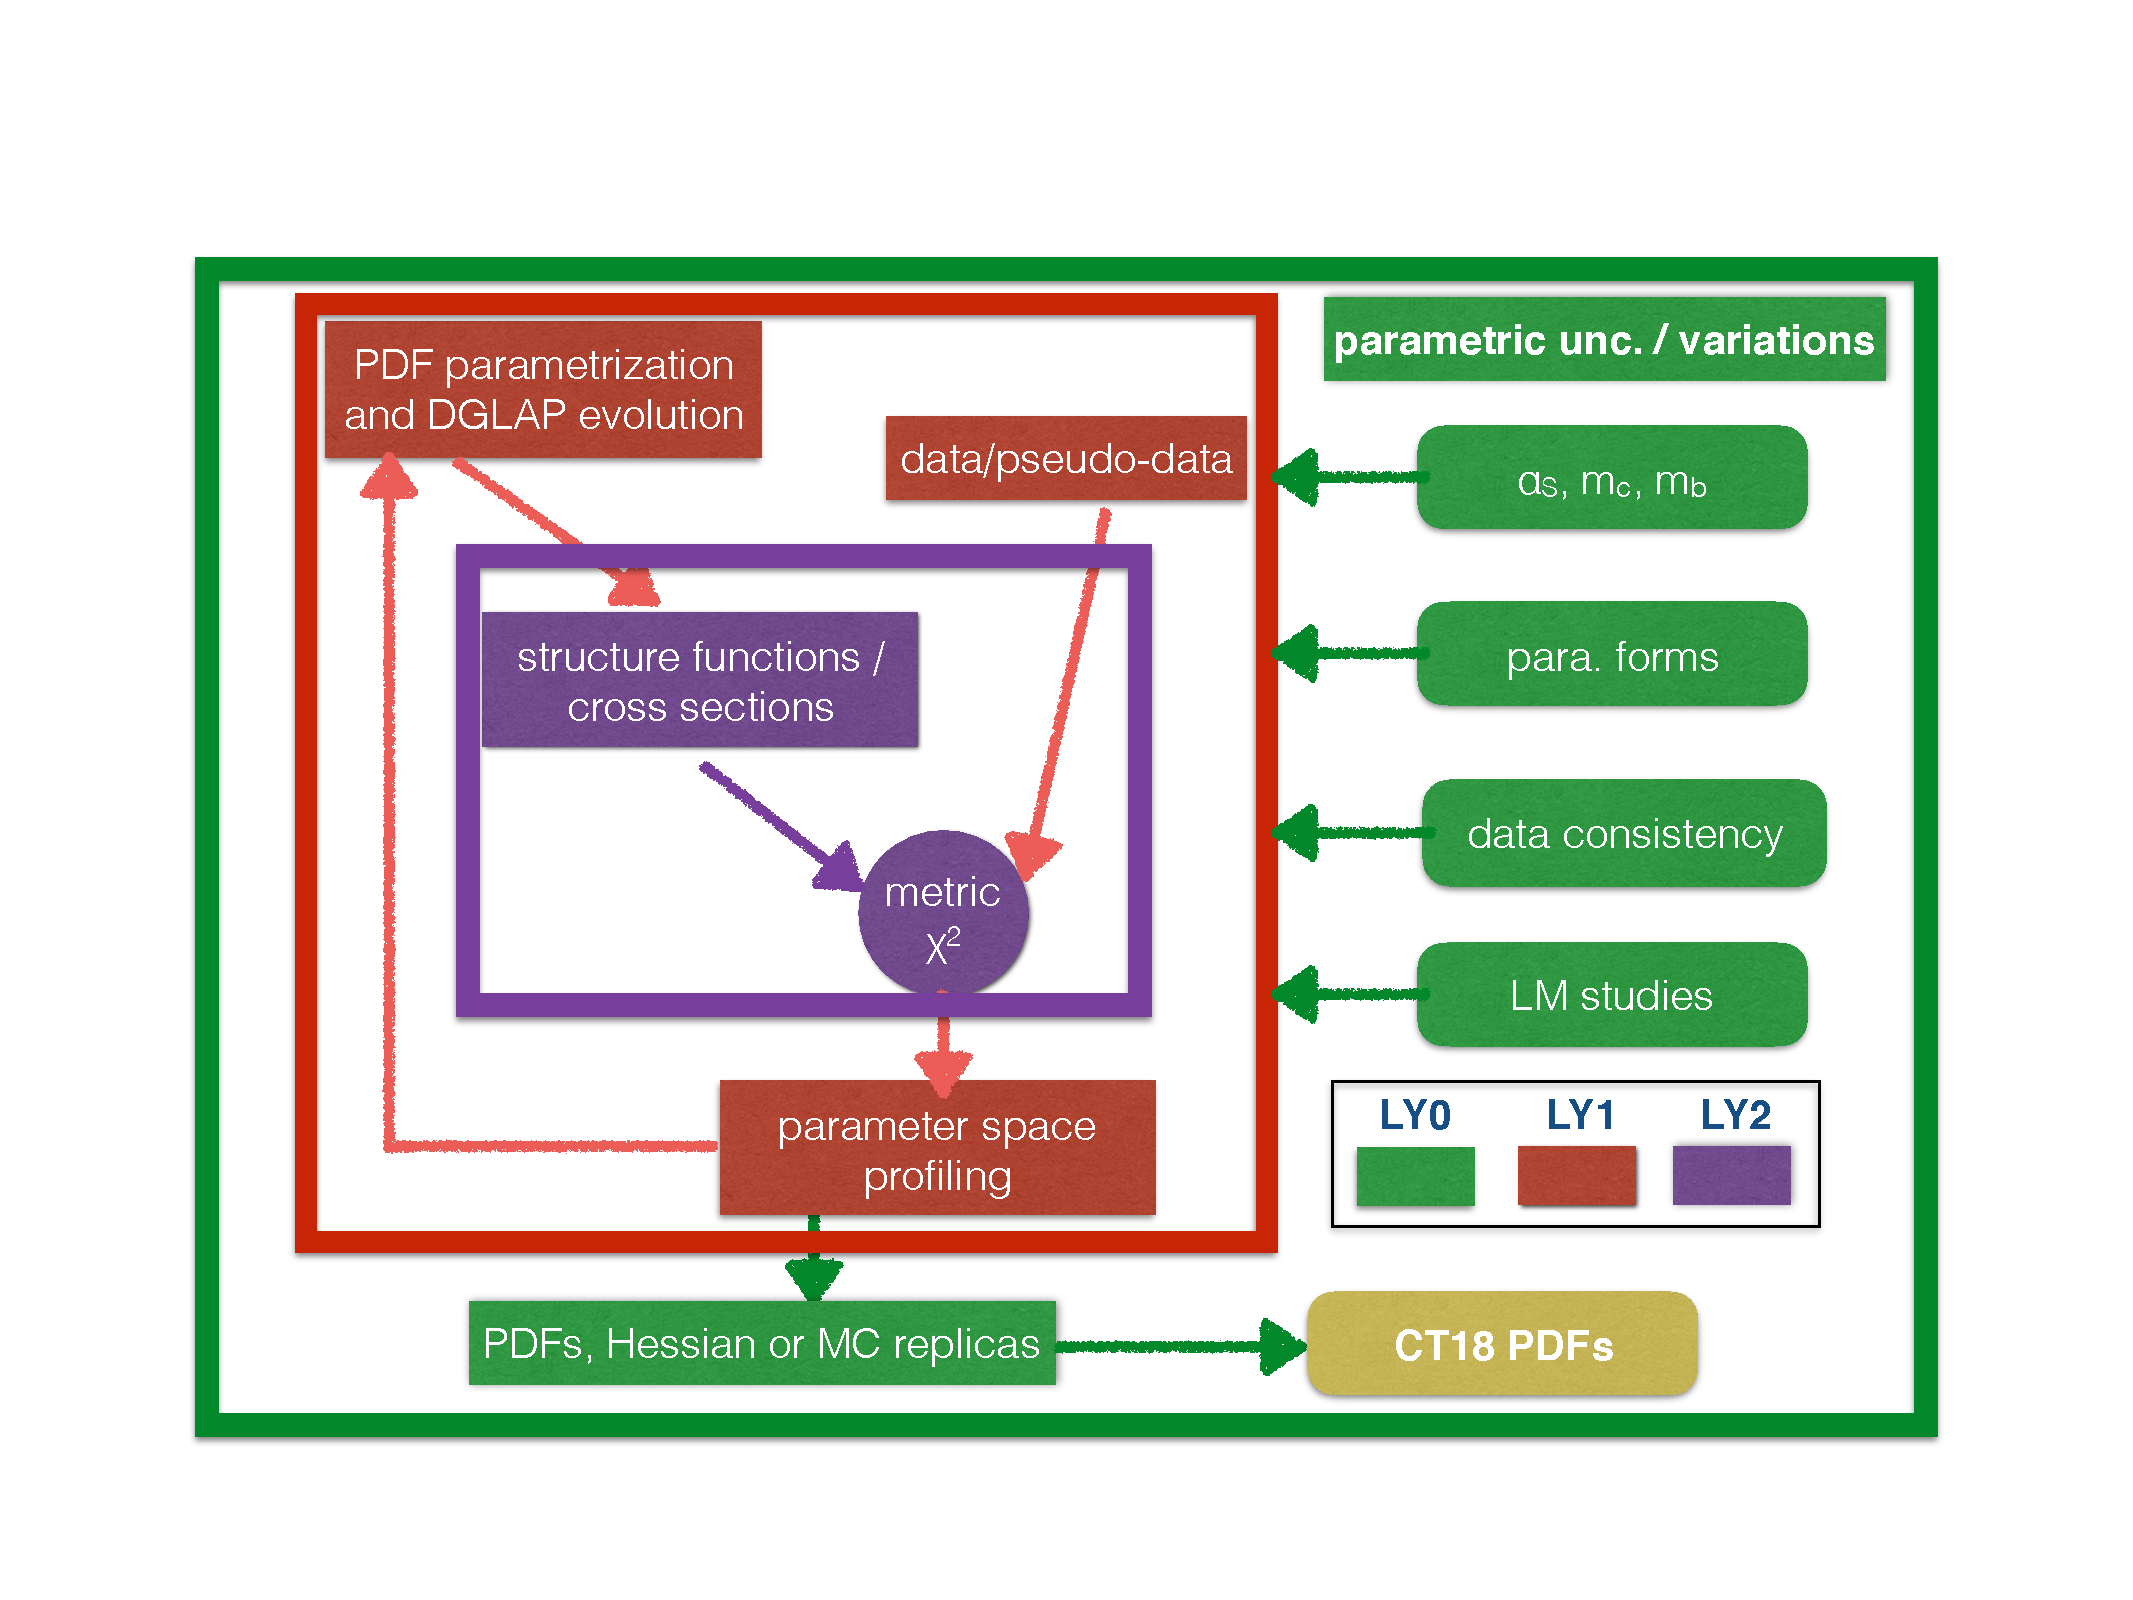
\includegraphics[width=0.99\textwidth]{./fig/CT18code.pdf}
	\end{center}
	\vspace{-2ex}
	\caption{\label{fig:gfit}
		%
		A flowchart of the CT18 global analysis consists of the outer layer (LY0),
		middle layer (LY1), and core process (LY2).
	}
\end{figure}

%
Within the LY1 layer, the calculation of global $\chi^2$, or "layer LY2", is the core part of the fit that will
be repeated for every combination of the PDF parameters.
%
LY2 calculates cross sections for thousands of data points and computes individual $\chi^2$ for each data set. 


%
Most computational efforts shown in Fig.~\ref{fig:gfit} can be parallelized.
For instance, at the LY0 stage, one can simply submit thousands of simultaneous fits with varied inputs to a large computing cluster, since those fits are
independent. To obtain a diverse battery of results presented in the CT18(Z) analyses, including the computationally expensive Lagrange Multiplier scans, the high-performance computing clusters at MSU and SMU were used. 

%
At LY1, the major task is to find a global minimum of the $\chi^2$ in a parameter space with large dimensions ($N_{par}\sim 30$).
The choice of the suitable parallelization technique depends strongly on the minimization algorithm.
%
The CT18 analysis uses the variable-metric gradient descent method implemented in the \texttt{MINUIT} package~\cite{James:2004xla}.
%
It involves numerical calculations of the first- and 
second-order derivatives of $\chi^2$, combined with sequential minimum searches along fixed directions
in the PDF parameter space.
%
The calculations of derivatives are highly parallelizable, with the CPU-time expenditures scaling with the number $N_{par}$ of parameters approximately as
$1/N_\mathit{par}$ and $2/(N^2_\mathit{par}\!+\!N_\mathit{par})$, respectively.

%
In the core part, again the calculation of individual $\chi^2$ for different data sets, including their cross sections, is now done simultaneously.
While either \texttt{MPI} or \texttt{OpenMP} parallelization protocols are suitable at this stage,
the latter is restricted to platforms with shared memory, but required fewer revisions in our fitting code.
%
Specifically, we used an approach similar to \texttt{OpenMP} to reduce the scope of changes inside
our fitting code.
%
When computing $\chi^2_E$ values for the experiments, the \verb|fork| Linux command splits the main program into multiple threads,
each with a copy of the master memory and carrying out the calculations independently.
%
Later the \verb|join| command collects the  results from the individual threads and returns them to
the main program.
%
The implementation of this \verb|fork-join| algorithm is borrowed from the widely-used
CUBA library~\cite{Hahn:2004fe} for multi-thread Monte-Carlo integration.   

\section{Decorrelation of ATLAS jet-production cross-section data}
\label{sec:ATLASjetdecorrel}
%
%
It has been observed in our global analysis, as well as others \cite{Harland-Lang:2017ytb}, that achieving a robust theoretical description of the Run-1 LHC jet production data generally requires numerical prescriptions to decorrelate select correlated systematic uncertainties. In our work, we follow the recommendations of experimental collaborations in applying such decorrelation procedures.


%
%
For example, while the ATLAS 7 TeV inclusive jet production data \cite{Aad:2014vwa} (Exp.~ID=544) produced an unacceptably high $\chi^2$ when fitted out of the box, the agreement of data and NNLO theory was improved by applying some decorrelation options
proposed by the ATLAS collaboration and summarized in the Appendix of Ref.~\cite{Aaboud:2017dvo}. 
The CT18(Z) fits implement ATLAS inclusive jet cross sections defined with an $R=0.6$ anti-$k_t$ jet algorithm. With this data set, we tested
the decorrelation procedures summarized in Table 6 of Ref.~\cite{Aaboud:2017dvo} and 
found some to have a substantial impact on the $\chi^2_E/N_\mathit{pt,E}$ of the ATLAS 7 TeV data. In the end, we followed the specific recommendations
of the ATLAS experimentalists themselves, who advocate \cite{Bogdan} the decorrelation of two jet energy scale (JES) uncertainties, associated with the JES MJB fragmentation (JES16) and the JES flavor response
(JES62). We obtained the greatest $\chi^2$ reduction using the upper portion of Table~6 in Ref.~\cite{Aaboud:2017dvo},
by decorrelating JES16 and JES62 according to Options 17 and 14 of Table~4, respectively. 

Ref.~\cite{Aaboud:2017dvo}
also details decorrelation options for select uncertainties in experimental simulations; 
of these, we specifically considered the effect of
decorrelating the error associated with the nonperturbative correction (`eNPC'), but found it to have negligible impact
on the quality of the \CTHERAII~fit according to $\chi^2$. 

The JES decorrelation that we have implemented proceeds by breaking a given correlated uncertainty into 2-3 subsidiary errors such that their sum in quadrature recovers the original correlated uncertainty. This procedure is bin-dependent; the resulting decorrelated
errors depend on the jet's rapidity and transverse momentum. For example, we decorrelate the JES MJB fragmentation error, $\delta_{16}$, into
three components given by
%
\begin{align}
	\delta^a_{16} &= \delta_{16}\, \Big\{ 1 - L^2\big( \ln(p_T[\mathrm{TeV}]),\ln(0.1),\ln(2.5) \big) \Big\}^{1/2}\, \left( 1 - L^2\big(|y|,0,1\big) \right)^{1/2}, \nonumber \\
	%
	\delta^b_{16} &= \delta_{16}\, \Big\{ 1 - L^2\big( \ln(p_T[\mathrm{TeV}]),\ln(0.1),\ln(2.5) \big) \Big\}^{1/2}\, L\big(|y|,1,3\big), \nonumber \\
	%
	\delta^c_{16} &= \big( \delta^2_{16} - (\delta^a_{16})^2 - (\delta^b_{16})^2 \big)^{1/2}\ ,
\label{eq:dec16}
\end{align}
%
where
%
\begin{equation}
L(x,x_\mathit{min},x_\mathit{max}) \equiv \frac{x - x_\mathit{min}}{x_\mathit{max} - x_\mathit{min}}\ \iff x \in [x_\mathit{min},x_\mathit{max}]\ ,
\end{equation}
%
and otherwise $L = 0$ for $x < x_\mathit{min}$ or $L = 1$ for $x > x_\mathit{max}$. We note that Eq.~(\ref{eq:dec16}) governs the magnitudes of the decorrelated uncertainties, which otherwise
inherit the sign of the original uncertainty. A similar algorithm is applied to decorrelate the JES flavor response JES62.

{\color{red} Tim:
Analogous considerations were applied to the inclusive jet production data sets from CMS 7 and 8 TeV (experiments 542 and 545).  Namely, for the 7 TeV CMS jet data, the decorrelation methods of
Ref.~\cite{Khachatryan:2014waa} were applied to JEC2 with an additional
decorrelation\footnote{Private communication, Voutilainen.} for the $2.5 < |y| < 3.0$ bin to obtain 6 subsidiary uncertainties. For the 8 TeV CMS jet data, systermatic uncertainties
were obtained using the xFitter framework according to the treatment in Ref.~\cite{Khachatryan:2016kdb}.
}
%
On the top of that, we found that the residual fluctuations
from the Monte-Carlo integration of the available NNLO predictions from \texttt{NNLOJet} \cite{Ridder:2015dxa,Gehrmann-DeRidder:2017mvr,Currie:2016bfm,Currie:2017ctp} lead to elevated $\chi^2$ for the inclusive jet production experiments, or equivalently, to some uncertainty in the tabulated NNLO/NLO corrections if they are fitted by a smooth function.   
In the CT18 analysis, the Monte-Carlo (MC) theoretical uncertainty for the three jet experiments is estimated by adding an overall {\it uncorrelated} uncertainty (`MC unc.') of 0.5\%, the typical magnitude of the intrinsic statistical noise associated with Monte-Carlo generation of NNLO/NLO $K$-factors. 
 
Table~\ref{tab-chi} summarizes the reduction in $\chi^2_E/N_{pt,E}$ for the three LHC jet data sets after performing the decorrelation and adding the Monte-Carlo uncertainties, on the example of the \CTHERAII~ PDFs. For example, for the ATLAS 7 TeV jet data, the decorrelation reduces $\chi^2_E$ by $\gtrsim\!\! 90$ units, yet adding the MC uncertainty is still necessary to reduce the $\chi^2_E/N_{pt,E}$ to a statistically plausible level (from 1.68 to 1.31 for $N_{pt,E}=140$). 

%
\begin{table}[tb]
	\begin{tabular}{c|ccc}
		\hline
		\hline
       	&	\multicolumn{3}{c}{evaluated, {\bf CT14$_\mathrm{HERAII}$ NNLO}} 	\ \ \ \\
		%%%
		\ \ \  $\chi^2_E/N_{pt,E}$ \ \ \	& \ \ \ original data \ \ \  &  \ \ \  $+$\,decorr. \ \ \    &  \ \ \  $+$\,0.5\% MC unc. \ \ \   \\
		\hline
		\ \ \ ATLAS, 7 TeV \ \ \   &  \ \ \  2.34 \ \ \   &  \ \ \  1.68 \ \ \   &  \ \ \  1.31 \ \ \   \\
		\ \ \ CMS, 7 TeV   \ \ \   &  \ \ \  1.58 \ \ \   &  \ \ \  1.45 \ \ \   &  \ \ \  1.35 \ \ \   \\
		\ \ \ CMS, 8 TeV   \ \ \   &  \ \ \  1.90 \ \ \   &  \ \ \  1.34 \ \ \   &  \ \ \  1.23 \ \ \   \\
		\hline
		\hline
	\end{tabular}
	\caption{Values of $\chi^2_E/N_{pt,E}$ for the inclusive jet production data implemented in CT18,
		computed here using the \CTHERAII~PDFs \cite{Hou:2016nqm} under several error treatment scenarios. $\chi^2_E/N_{pt,E}$ is first given without
		implementing any decorrelation scheme (``original data''); using the decorrelation scheme described
		above (``$+$\, decorr.''); and, finally, adding an overall uncorrelated Monte Carlo uncertainty of 0.5\% on the top of decorrelations ("$+$\,0.5\% MC unc.").
	}
	\label{tab-chi}
\end{table}

